%----------------------------------------------------------------------------------------
%----------------------------------------------------------------------------------------

% =====================================================================================================
%
%  EDA 	- 	Exploratory Data Analysis
%
% =====================================================================================================
\section{Missing \& Duplicate Observations}
\label{sec:EDA}

We observe an initial 97 samples in the \textit{crime\_v2.csv} file, as well as all 25 columns listed in the code book above.  An initial pass through the data reveals two obvious data-collection errors: (\textbf{a}) 6 empty rows at the tail of the file (see \ref{fig:Empty Rows}), and (\textbf{b}) one row that has been duplicated for county 193 (see \ref{fig:Duplicate Row}): \\

\begin{figure}[!ht]
	\begin{subfigure}[b]{1.0\textwidth}
		\centering
		\caption{6 rows with missing values at tail of file}
		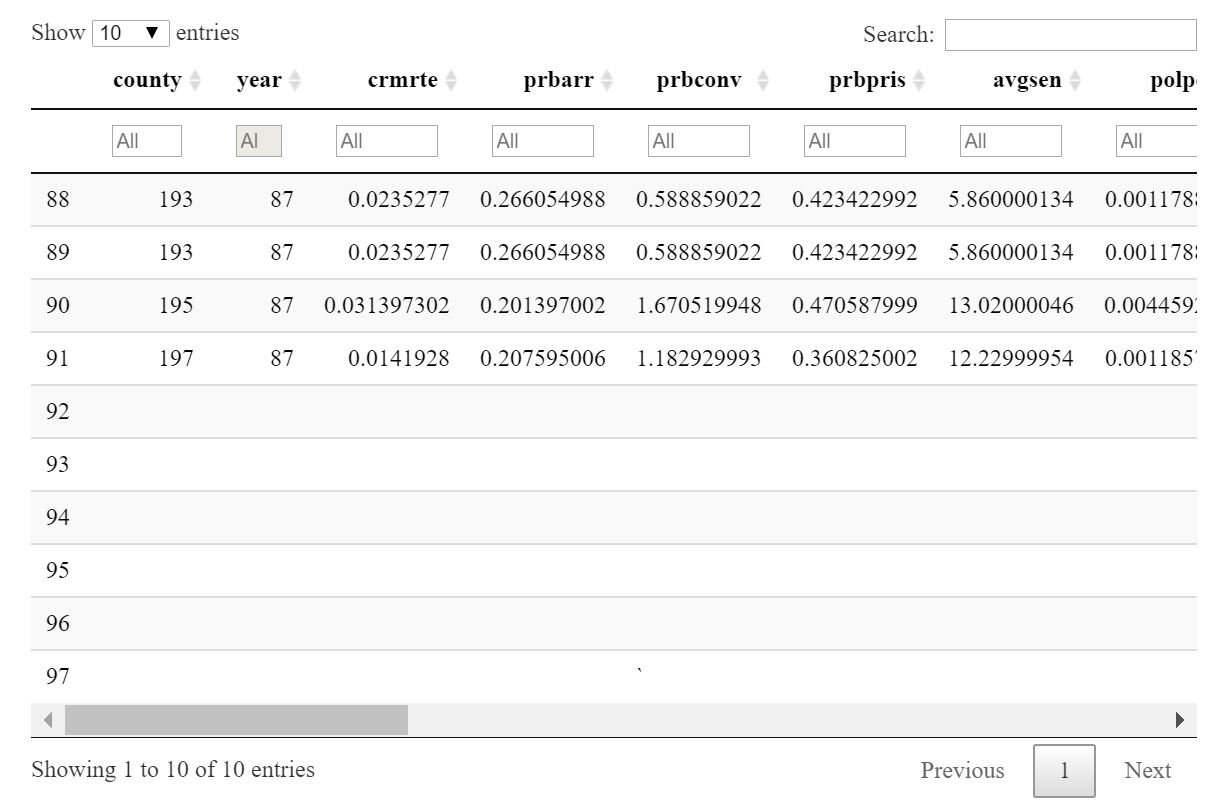
\includegraphics[width=\linewidth]{images/EDA_empty_rows.jpg}
		\label{fig:Empty Rows}
	\end{subfigure}\vspace{3mm}% or \hspace{0.3\textwidth}
	\hfill
	
	\begin{subfigure}[b]{1.0\textwidth}
		\centering
		\caption{Row for county 193 duplicated}
		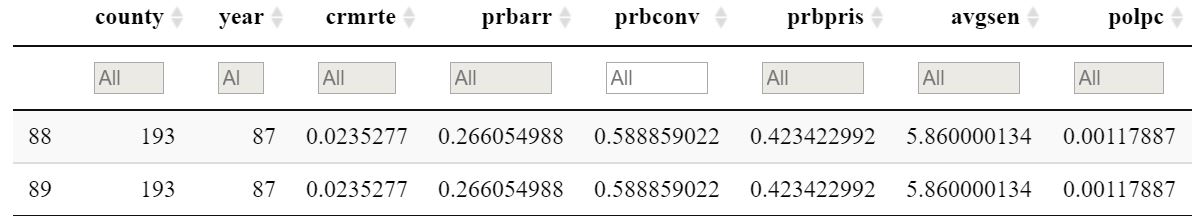
\includegraphics[width=\linewidth]{images/EDA_duplicate_rows.jpg}
		\label{fig:Duplicate Row}
	\end{subfigure}
	\label{fig:EDA Duplicate and Missing Rows}
	\caption{EDA : Duplicated and Missing Rows}
\end{figure}

\pagebreak

\section{Descriptive Statistics}
\label{sec:Descriptive Statistics}
%\textbf{\textcolor{OrangeRed}{EXPLORATORY DATA ANALYSIS - CONTD.}}\\

Following removal of six empty rows and one of the duplicate rows, we are left with 90 observations useful for analysis.  The descriptive statistics for the variables of interest were captured:\\

\begin{table}[!htbp] 
	\centering 
	\small
	\caption{EDA : Descriptive Statistics} 
	\label{EDA - Descriptive Statistics} 
	\begin{tabular}{@{\extracolsep{5pt}}lccccccc} 
		\\[-1.8ex]\hline 
		\hline \\[-1.8ex] 
		Statistic & \multicolumn{1}{c}{N} & \multicolumn{1}{c}{Mean} & \multicolumn{1}{c}{St. Dev.} & \multicolumn{1}{c}{Min} & \multicolumn{1}{c}{Pctl(25)} & \multicolumn{1}{c}{Pctl(75)} & \multicolumn{1}{c}{Max} \\ 
		\hline \\[-1.8ex] 
		county & 90 & 100.60 & 58.32 & 1 & 51.5 & 150.5 & 197 \\ 
		year & 90 & 87.00 & 0.00 & 87 & 87 & 87 & 87 \\ 
		crmrte & 90 & 0.03 & 0.02 & 0.01 & 0.02 & 0.04 & 0.10 \\ 
		prbarr & 90 & 0.30 & 0.14 & 0.09 & 0.20 & 0.34 & 1.09 \\ 
		prbconv & 90 & 0.55 & 0.35 & 0.07 & 0.34 & 0.59 & 2.12 \\ 
		prbpris & 90 & 0.41 & 0.08 & 0.15 & 0.36 & 0.46 & 0.60 \\ 
		avgsen & 90 & 9.69 & 2.83 & 5.38 & 7.38 & 11.47 & 20.70 \\ 
		polpc & 90 & 0.002 & 0.001 & 0.001 & 0.001 & 0.002 & 0.01 \\ 
		density & 90 & 1.44 & 1.52 & 0.0000 & 0.55 & 1.57 & 8.83 \\ 
		taxpc & 90 & 38.16 & 13.11 & 25.69 & 30.73 & 41.01 & 119.76 \\ 
		west & 90 & 0.24 & 0.43 & 0 & 0 & 0 & 1 \\ 
		central & 90 & 0.38 & 0.49 & 0 & 0 & 1 & 1 \\ 
		urban & 90 & 0.09 & 0.29 & 0 & 0 & 0 & 1 \\ 
		pctmin80 & 90 & 25.71 & 16.98 & 1.28 & 10.02 & 38.18 & 64.35 \\ 
		wcon & 90 & 285.35 & 47.75 & 193.64 & 250.75 & 314.98 & 436.77 \\ 
		wtuc & 90 & 410.91 & 77.36 & 187.62 & 374.33 & 440.68 & 613.23 \\ 
		wtrd & 90 & 210.92 & 33.87 & 154.21 & 190.71 & 224.28 & 354.68 \\ 
		wfir & 90 & 321.62 & 54.00 & 170.94 & 285.56 & 342.63 & 509.47 \\ 
		wser & 90 & 275.34 & 207.40 & 133.04 & 229.34 & 277.65 & 2,177.07 \\ 
		wmfg & 90 & 336.03 & 88.23 & 157.41 & 288.60 & 359.89 & 646.85 \\ 
		wfed & 90 & 442.62 & 59.95 & 326.10 & 398.78 & 478.26 & 597.95 \\ 
		wsta & 90 & 357.74 & 43.29 & 258.33 & 329.27 & 383.15 & 499.59 \\ 
		wloc & 90 & 312.28 & 28.13 & 239.17 & 297.23 & 328.78 & 388.09 \\ 
		mix & 90 & 0.13 & 0.08 & 0.02 & 0.08 & 0.15 & 0.47 \\ 
		pctymle & 90 & 0.08 & 0.02 & 0.06 & 0.07 & 0.08 & 0.25 \\ 
		\hline \\[-1.8ex] 
	\end{tabular} 
\end{table} 

From the descriptive statistics, we note several potential areas of concern and interest.  First, the $\textcolor{Blue}{county}$ variable appears to be the EPA FIPS code for \href{https://en.wikipedia.org/wiki/List_of_counties_in_North_Carolina}{North Carolina counties}.  The values are odd numbered only and from Figure \ref{fig:LocationCorrectedMap} (below) we can see that the Central/West/East indicators provided in the data geographically aligns using these values as FIPS codes.\\

Additionally, the variables $\textcolor{Blue}{wser}$,  $\textcolor{Blue}{density}$, $\textcolor{Blue}{polpc}$, $\textcolor{Blue}{taxpc}$, and $\textcolor{Blue}{pctymle}$ all appear to have a distribution that suggest potential outliers.  We will explore these variables to see if there may be more issues in the data collection that we can address.

\pagebreak
\section{Outlier Analysis}
\label{sec:Outliers}

\subsection{Weekly Wage, Service Industry [WSER]}

We start with $\textcolor{Blue}{wser}$, which appears to be the \textit{average weekly income for service industry workers}.  There exists a single large maximum value of $2177.07$ which appears to be well outside the distribution of the other values (see \ref{fig:EDA WSER variable uncorrected}).  The remaining values appear to be in the range of 133-348, so it seems very unlikely that only one county has a value in the 2,000+ weekly range (\$104,000 / year) for the service industry.  The county tied to this record is 185, which is the FIPS code for \href{https://en.wikipedia.org/wiki/Warren_County,_North_Carolina}{Warren County, North Carolina}.\\

This value appears to be the result of a decimal placement issue, where the likely real value is $217.7068$, based on a survey of the counties surrounding Warren County: Vance County ($347.6609$), Franklin County ($239.2233$), Nash County ($305.7612$), Halifax County ($172.6281$), and Northampton County ($213.5822$).  Given these surrounding county wages for service industry professionals, we come to a regional mean average of $\$255.7711$:\\

\textmathbf{
\begin{equation*}
\begin{aligned}
\mu_{regional\_wser} &= \frac{Vance + Franklin + Nash + Halifax + Northampton}{n}\\
&= \frac{\textcolor{Purple}{347.6609 + 239.2233 + 305.7612 + 172.6281 + 213.5822}}{5} = \frac{1278.856}{5}\\
\therefore &= \textcolor{OrangeRed}{255.7711}
\end{aligned}
\end{equation*}
}

Given these results, we elect to remediate the large outlier in $\textcolor{Blue}{wser}$ by multiplying the value by $0.1$.  The impact to distribution of values is depicted in \ref{fig:EDA WSER variable corrected} below:\\

\begin{figure}[!ht]
	\begin{subfigure}[t]{0.5\textwidth}
		\centering
		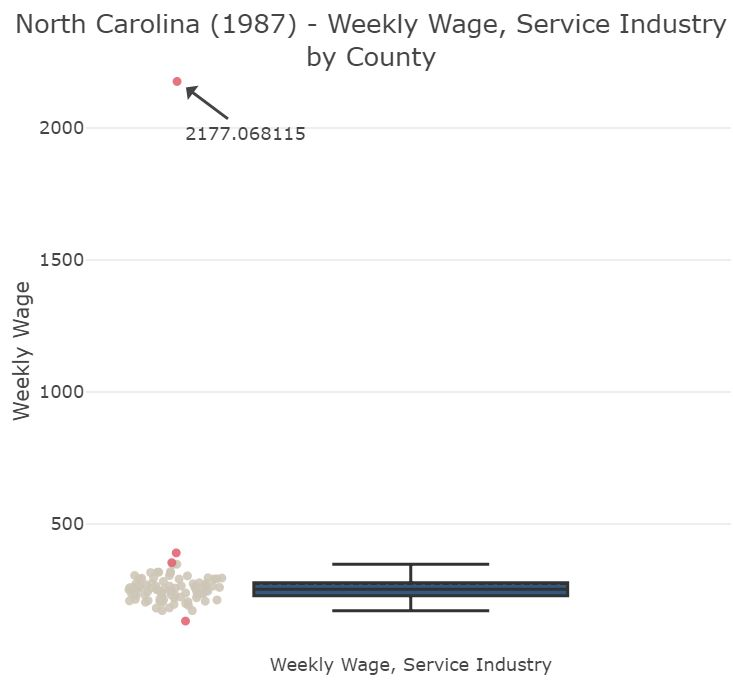
\includegraphics[width=\linewidth,height=3in]{images/EDA_wser_uncorrected.jpg}
		\caption{WSER with uncorrected, large outlier}
		\label{fig:EDA WSER variable uncorrected}
	\end{subfigure}
	\hfill
	\begin{subfigure}[t]{0.5\textwidth}
		\centering
		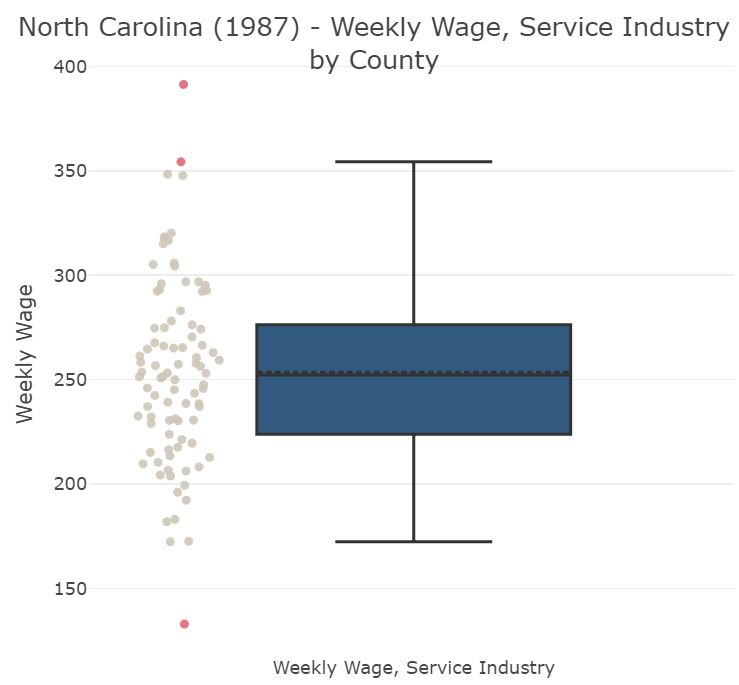
\includegraphics[width=\linewidth,height=3in]{images/EDA_wser_corrected.jpg}
		\caption{WSER with large outlier corrected}
		\label{fig:EDA WSER variable corrected}
	\end{subfigure}
	\caption{Outliers : Weekly Wage, Service Industry (WSER)}
	\label{fig:EDA WSER Outlier Treatment}
\end{figure}

\pagebreak

\subsection{People per Square Mile [DENSITY]}

Observation 79 (county = 173, \href{http://www.swaincountync.gov/}{Swain County}) is currently listed with a $\textcolor{Blue}{density}$ of of 0.0000203422 people per square mile.  By a wide-margin, this is the lowest value in the dataset (see \ref{fig:EDA DENSITY variable uncorrected}) and appears to be a potential mistake.  According to Wikipedia, \href{https://en.wikipedia.org/wiki/Swain_County,_North_Carolina}{Swain County} has a landmass of 541 square miles, which would equal 0.011 people living in the entire county - an impossibility.  \\

According to \href{https://www.google.com/publicdata/explore?ds=kf7tgg1uo9ude_&met_y=population&idim=county:37173&hl=en&dl=en}{U.S. Census Bureau records}, Swain County North Carolina had a population of 10,932 in 1987.  Upon reviewing $\textcolor{Blue}{density}$ more closely along with the Census Bureau records for population and the square mile landmass reported on Wikipedia, it appears that \textcolor{OrangeRed}{\textit{this variable is actually in units of 100 people per square mile}}.  With that adjustment, the data for Swain County would still equal only 1.1 person for the entire county; which is still clearly incorrect.\\

Based on the adjusted amount of 109.32 persons (in units of 100), the correct $\textcolor{Blue}{density}$ value for Swain County in 1987 should be $0.202070$.  We adjust accordingly (see \ref{fig:EDA DENSITY variable corrected}):\\

\vspace*{0.5in}
\begin{figure}[!ht]
	\begin{subfigure}[t]{0.5\textwidth}
		\centering
		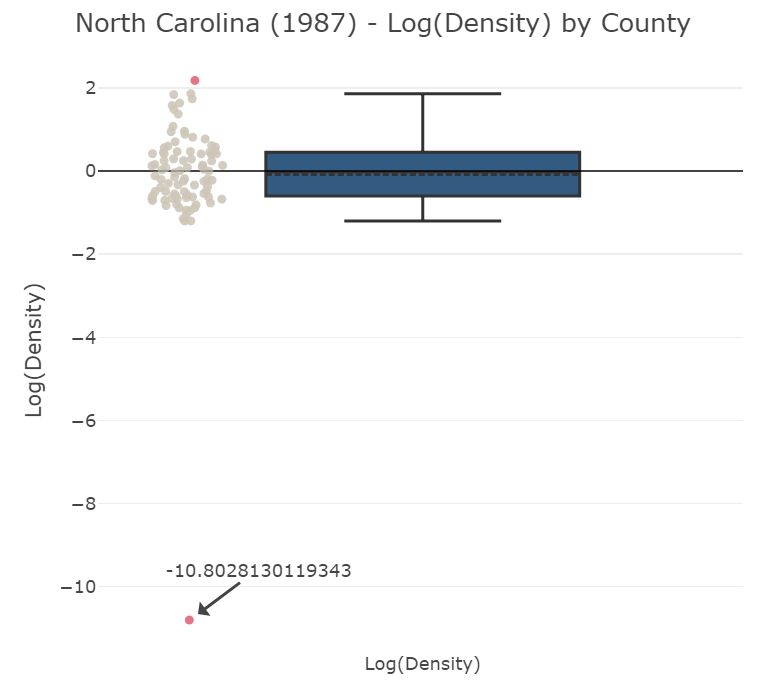
\includegraphics[width=\linewidth,height=3.5in]{images/EDA_density_uncorrected.jpg}
		\caption{log(density) with uncorrected, small outlier}
		\label{fig:EDA DENSITY variable uncorrected}
	\end{subfigure}
	\hfill
	\begin{subfigure}[t]{0.5\textwidth}
		\centering
		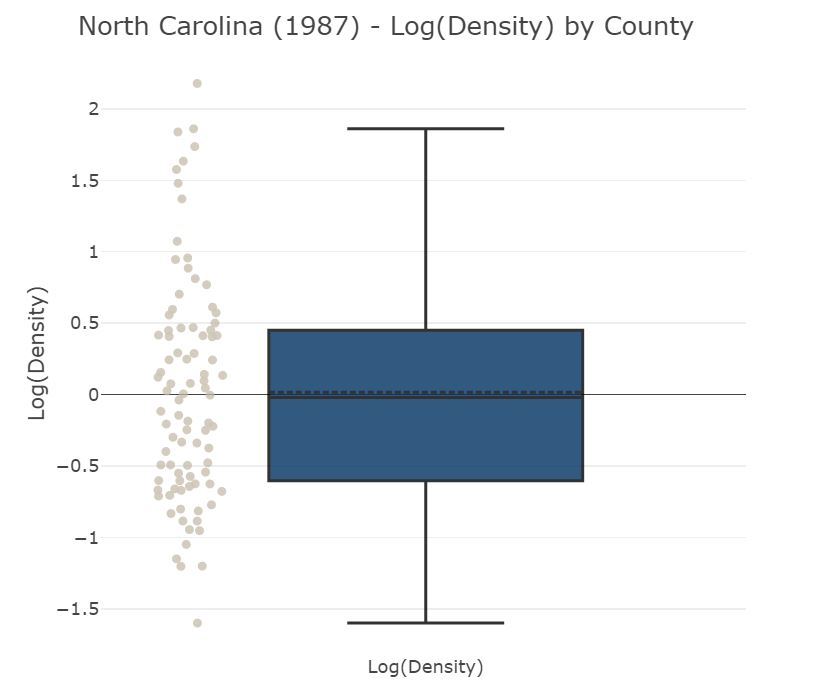
\includegraphics[width=\linewidth,height=3.5in]{images/EDA_density_corrected.jpg}
		\caption{log(density) with small outlier, corrected}
		\label{fig:EDA DENSITY variable corrected}
	\end{subfigure}
	\label{fig:EDA DENSITY Outlier Untreaded and Treated}
	\caption{Outliers : People per Square Mile (DENSITY)}
\end{figure}

\pagebreak

\subsection{Police per Capita [POLPC]}

There are a total of five data points in the $\textcolor{Blue}{polpc}$ variable that qualify as anomalous (\href{https://en.wikipedia.org/wiki/Outlier}{IQR Rule}), but one stands well above the others and warrants additional scrutiny.  The entry for county 115 (\href{https://www.madisoncountync.gov/}{Madison County}) has a value of $0.00905433$ (see \ref{fig:EDA POLPC variable uncorrected}), significantly higher than the other values in all other counties.  According to the \href{https://www.google.com/publicdata/explore?ds=kf7tgg1uo9ude_&met_y=population&idim=county:37173&hl=en&dl=en#!ctype=l&strail=false&bcs=d&nselm=h&met_y=population&scale_y=lin&ind_y=false&rdim=country&idim=county:37115&ifdim=country&hl=en_US&dl=en&ind=false}{U.S. Census}, Madison County, NC had a population size of only 17,051 residents in 1987 making it one of the smaller counties in the state overall.  Madison County covers only 452 square miles of geography and is located in the Northwest portion of the state, directly bordering Tennessee.\\

At this per capita level, Madison County would have $154.38538$ officers covering just 17,051 people.  The mean of the $\textcolor{Blue}{polpc}$ variable is $0.00162543$ (excluding Madison County); with this value substituted for Madison, we would have a more realistic level of $\approx 27.715$ law enforcement officers, which is in-line with other counties in the 20k and below population range.  We'll substitute with the mean for Madison County to address this apparent mistake; \ref{fig:EDA POLPC variable corrected} reflects the data distribution following the adjustment:\\

\vspace*{0.5in}
\begin{figure}[!ht]
	\begin{subfigure}[b]{0.5\textwidth}
		\centering
		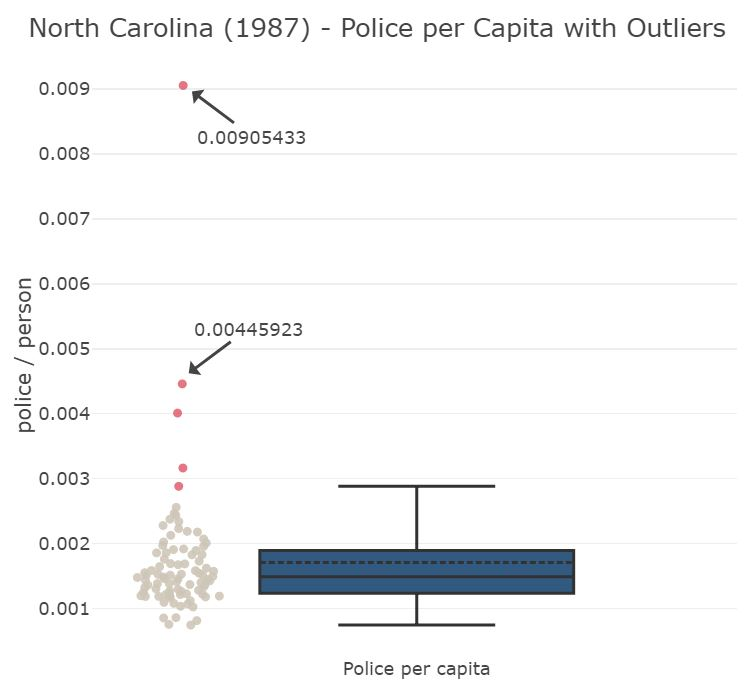
\includegraphics[width=\linewidth]{images/EDA_polpc_uncorrected.jpg}
		\caption{POLPC with uncorrected, large outlier}
		\label{fig:EDA POLPC variable uncorrected}
	\end{subfigure}
	\hfill
	\begin{subfigure}[b]{0.5\textwidth}
		\centering
		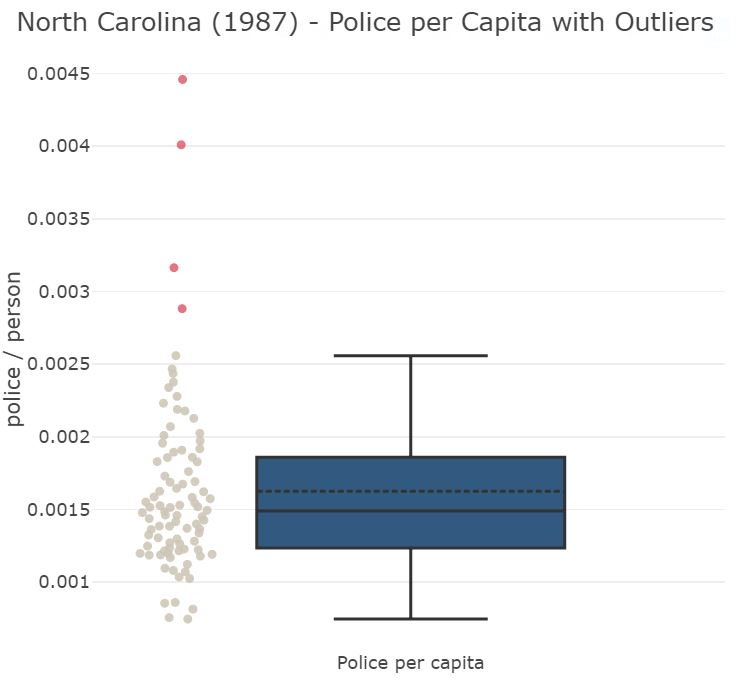
\includegraphics[width=\linewidth]{images/EDA_polpc_corrected.jpg}
		\caption{POLPC with large outlier corrected}
		\label{fig:EDA POLPC variable corrected}
	\end{subfigure}
	\label{fig:EDA POLPC Outlier Treatment}
	\caption{Outliers : Police per Capita (POLPC)}
\end{figure}

\pagebreak

\subsection{Tax Revenue per Capita [TAXPC]}

Next, we analyze a single large outlier found in the $\textcolor{Blue}{taxpc}$ variable.  According to the code book (ref: \ref{fig:Code Book}), $\textcolor{Blue}{taxpc}$ is the tax revenue per capita and while the typical range is from 25 - 75, county 55 (\href{https://www.darenc.com/}{Dare County}) has a large value of $119.76$ per person.  In 1987, Dare County had a population of 19,580 according to \href{https://www.google.com/publicdata/explore?ds=kf7tgg1uo9ude_&met_y=population&idim=county:37055:37053&hl=en&dl=en}{U.S. Census records}.  The tax rate in Dare County is roughly the same as other counties at 2\% with a total state + county combined rate of 6.75\%.\\

Based on the historical tax rates and the increasing burden we see in NC taxes from 1981-1987 \href{https://www.ncleg.gov/DocumentSites/committees/FiscalModernization/Comission\%20Meetings/Nov\%2028\%20and\%2029/Nov\%2028\%20Presentations/History\%20of\%20State\%20and\%20Local\%20Taxes\%20in\%20NC\%20Paper.pdf}{(reference)}, it is not clear if the value reported in the data is incorrect.  As such, we elect not to treat this value and leave it as-is for the purposes of our analysis.\\

\vspace*{0.5in}
\begin{figure}[!ht]
\centering
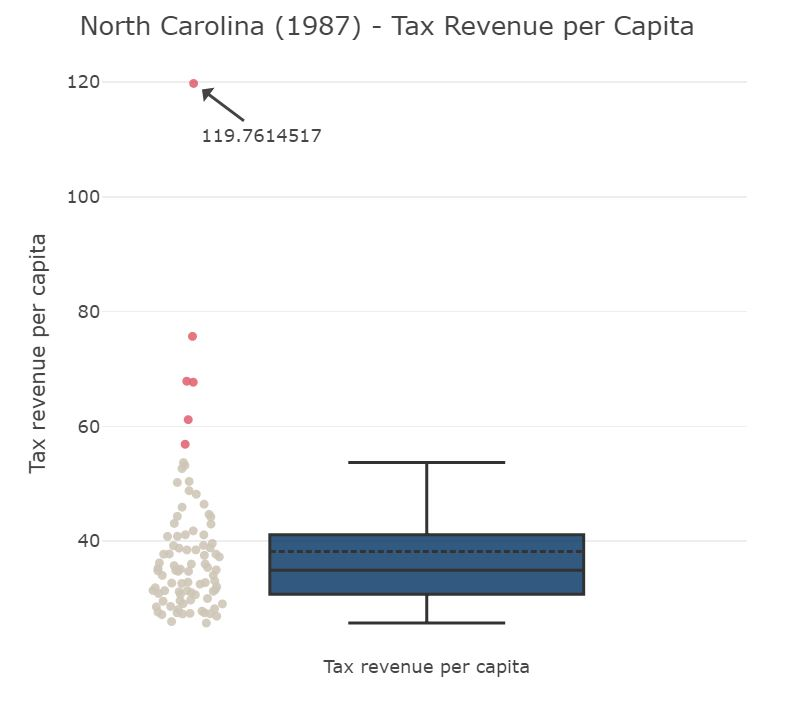
\includegraphics{images/EDA_taxpc_uncorrected.jpg}
\label{fig:EDA TAXPC variable uncorrected}
\caption{Outliers : Tax Revenue per Capita (TAXPC)}
\end{figure}

\pagebreak

\subsection{Percentage of Demographic as Young Males [PCTYMLE]}

We analyze a single large outlier found in the $\textcolor{Blue}{pctymle}$ variable.  According to the code book (ref: \ref{fig:Code Book}), $\textcolor{Blue}{pctymle}$ is the percent of young males representing the county population.  County 133 (\href{https://www.onslowcountync.gov/}{Onslow County}) has a relatively large value of almost 25\%, warranting further investigation.  According to Wikipedia, \href{https://en.wikipedia.org/wiki/Onslow_County,_North_Carolina}{Onslow County} is home to the U.S. Marine Corps Base \href{https://www.lejeune.marines.mil/}{Camp Lejeune}.\\

Though women have been permitted to join the U.S. Marines since 1918, historically they have made up less than 10\% of all U.S. Marines roles \href{https://en.wikipedia.org/wiki/Women_in_the_United_States_Marines}{(reference)}. It was not until calendar year 2016 that women were allowed to serve in all roles.  In addition to this, contemporary demographics statistics report that the median age of Onslow County is 25 \href{https://en.wikipedia.org/wiki/Onslow_County,_North_Carolina}{(reference)}.  Given these data, \textcolor{OrangeRed}{\textit{we conclude that this large value is accurate}} and elect to leave it as-is for the purposes of this analysis.

\vspace*{0.5in}
\begin{figure}[!ht]
	\centering
	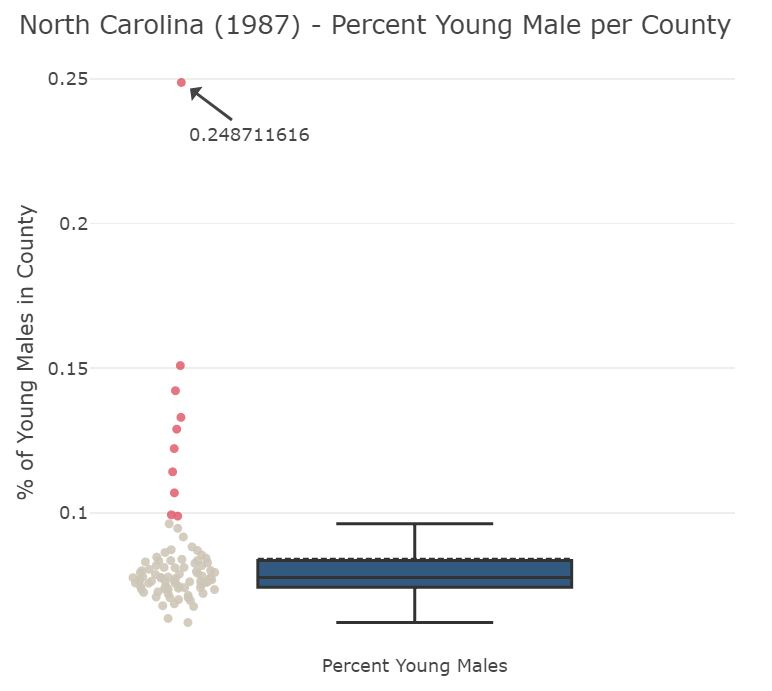
\includegraphics{images/EDA_pctymle_uncorrected.jpg}
	\label{fig:EDA PCTYMLE variable uncorrected}
	\caption{Outliers : Percentage of Demographic as Young Males (PCTYMLE)}
\end{figure}

\pagebreak

\section{Location Errata}

The use of one-hot encoding for location variables $\textcolor{Blue}{west}$ and $\textcolor{Blue}{central}$ is potentially problematic as it allows for the possibility of insert/update anomalies. That is, the form of the data allows for impossible assignments into more than one location.  The dataset we were provided with contains only one such anomaly for \href{http://www.gastongov.com/}{Gaston County} (FIPS code 71).  This variable has inadvertently been assigned to both the "Central" and "West" groups (see figures \ref{fig:EDA Location - Gaston County} and \ref{fig:EDA Location map - Gaston County}).\\

\begin{figure}[!ht]
	\begin{subfigure}[b]{0.5\textwidth}
		\centering
		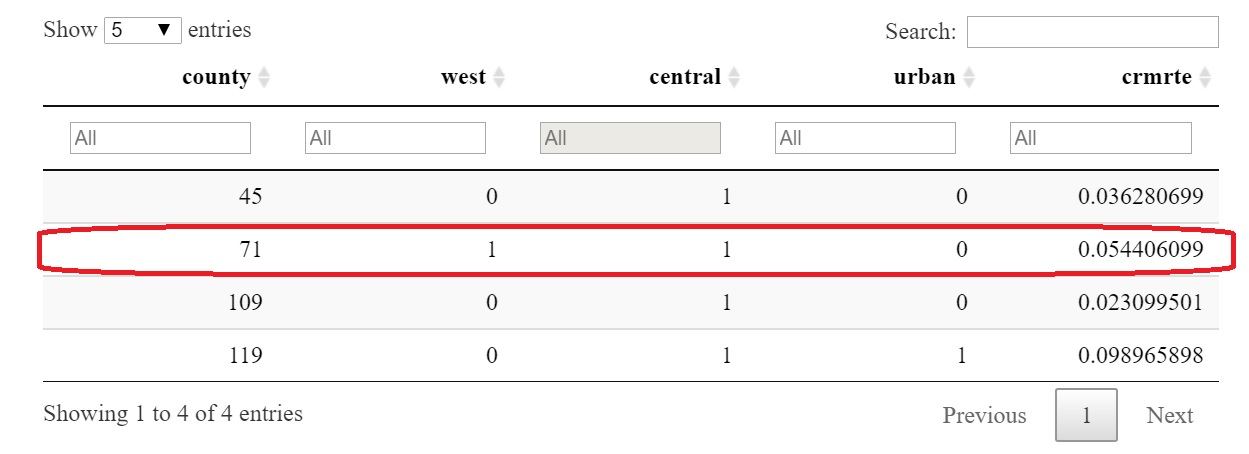
\includegraphics[width=\linewidth]{images/EDA_location_incorrect_category.jpg}
		\caption{Gaston County assigned to two location codes}
		\label{fig:EDA Location - Gaston County}
	\end{subfigure}
	\hfill
	\begin{subfigure}[b]{0.5\textwidth}
		\centering
		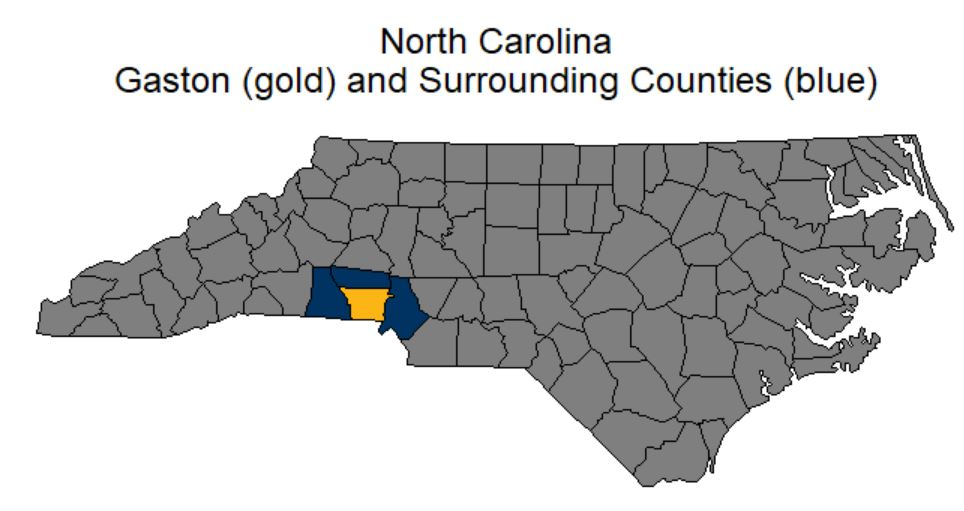
\includegraphics[width=\linewidth]{images/EDA_location_map.jpg}
		\caption{Gaston and surrounding counties}
		\label{fig:EDA Location map - Gaston County}
	\end{subfigure}
	\caption{EDA : Location Category of Gaston County}
	\label{fig:Local Errata}
\end{figure}

\href{http://www.gastongov.com/}{Gaston County} is surrounded by only three North Carolina counties:  \href{https://www.clevelandcounty.com/main/}{Cleveland County} to the West, \href{https://www.lincolncounty.org/}{Lincoln County} to the North, and \href{https://www.mecknc.gov/Pages/Home.aspx}{Mecklenburg County} to the East.  In this case, all of the surrounding counties are labeled as members of the "Central" category, so \textcolor{OrangeRed}{we correct the value for Gaston by removing it from the "West" category, leaving it assigned to "Central"}.  Following this correction, all counties appear to be distributed uniformly (see \ref{fig:LocationCorrectedMap})\\

\begin{figure}[!ht]
	\centering
	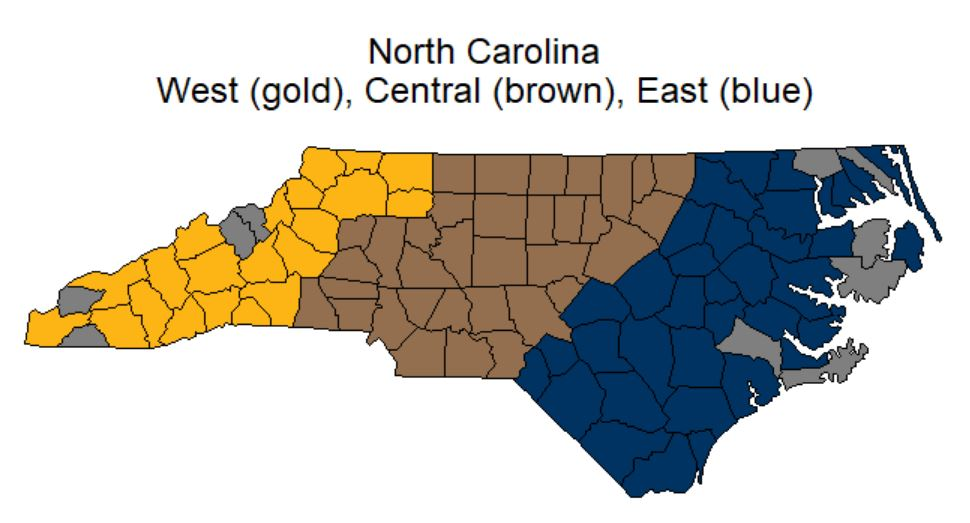
\includegraphics[scale=0.9]{images/EDA_location_map_correct.jpg}
	\caption{EDA : North Carolina Geographic Boundaries (West, Central, East)}
	\label{fig:LocationCorrectedMap}
\end{figure}

\pagebreak

\section{Crime Rate by County}

Earlier, we identified the $\textcolor{Blue}{county}$ variable as the FIPS code for North Carolina counties (ref \ref{sec:Descriptive Statistics}).  We can use this information to identify counties missing from our dataset as well as plot crime rates at a county level to see if there are any overt geographical signals of crime rate.\\

We received data for only 90 of the 100 counties in North Carolina; the missing counties are shown in Figure \ref{fig:MissingCountiesList}, and are identified geographically in Figure \ref{fig:MissingCountiesGraph} [in grey].

\begin{figure}[!ht]
	\small
	\begin{minipage}[t]{0.3\textwidth}
		\caption{EDA : Missing Counties}
		\begin{tabular}[t]{{p{1.0cm}p{3.0cm}}}
			\toprule
			\textbf{FIPS} & \textbf{County} \\
			\midrule
			29  &  Camden \\
			31  &  Carteret \\
			43  &  Clay \\
			73  &  Gates \\
			75  &  Graham \\
			95  &  Hyde \\
			103  &  Jones \\
			121  &  Mitchell \\
			177  &  Tyrrell \\
			199  &  Yancey \\
			\bottomrule
		\end{tabular}
		\label{fig:MissingCountiesList}
	\end{minipage} \hfill
	\begin{minipage}[t]{0.7\textwidth}
		\centering
		\caption{EDA : North Carolina Crime by County, 1987}
		\begin{subfigure}[t]{1.0\textwidth}
			\centering
			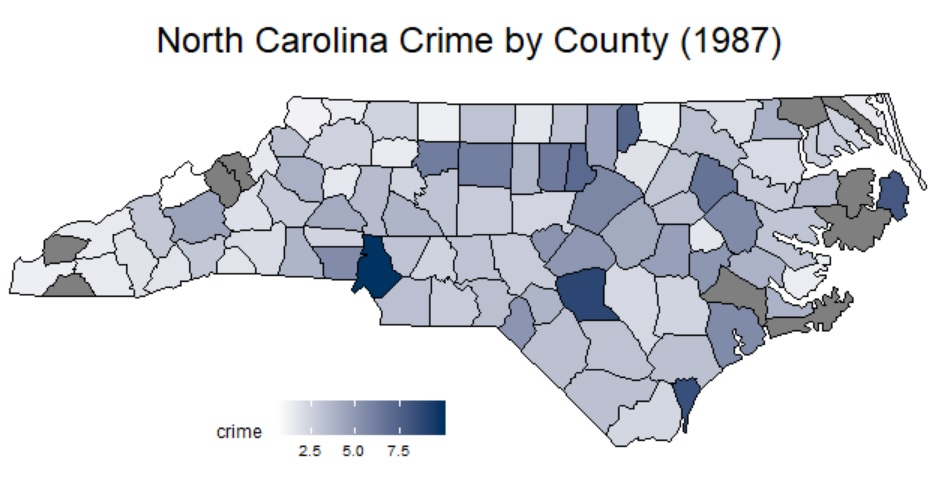
\includegraphics[width=\linewidth]{images/EDA_crmrte_by_county.jpg}
		\end{subfigure}
		\label{fig:MissingCountiesGraph}
	\end{minipage}
\end{figure}

No apparent strong crime rate patterns exist from a purely visual geographic positioning perspective; however, it is noteworthy that counties with high crime rate per West/Central/East grouping \textit{in general} tends to increase moving West to East. \\

\begin{figure}[!ht]
	\label{fig:EDA : County Top and Bottom 10 Crime Rates}
	\begin{minipage}[t]{0.5\textwidth}
	\centering
	\caption{EDA : Top 10 Counties by Crime Rate}
	\begin{tabular}[t]{{p{1.0cm}p{3.0cm}p{2.5cm}}}
		\toprule
		\textbf{FIPS} & \textbf{County} & \textbf{Crime Rate} \\
		\midrule
		119 & Mecklenburg & $9.897 \%$ \\ 
		51 & Cumberland & $8.838 \%$ \\ 
		129 & New Hanover & $8.350 \%$ \\ 
		55 & Dare & $7.902 \%$ \\ 
		181 & Vance & $7.295 \%$ \\ 
		63 & Durham & $7.066 \%$ \\ 
		65 & Edgecombe & $6.588 \%$ \\ 
		135 & Orange & $6.290 \%$ \\ 
		67 & Forsyth & $6.142 \%$ \\ 
		81 & Guilford & $6.045 \%$ \\ 
		\bottomrule
	\end{tabular} 
	\end{minipage} \hfill
	\begin{minipage}[t]{0.5\textwidth}
	\centering
	\caption{EDA : Bottom 10 Counties by Crime Rate}
	\begin{tabular}[t]{{p{1.0cm}p{3.0cm}p{2.5cm}}}
		\toprule
		\textbf{FIPS} & \textbf{County} & \textbf{Crime Rate} \\
		\midrule
		117 & Martin & $0.553 \%$ \\ 
		9 & Ashe & $1.062 \%$ \\ 
		185 & Warren & $1.087 \%$ \\ 
		39 & Cherokee & $1.192 \%$ \\ 
		169 & Stokes & $1.210 \%$ \\ 
		137 & Pamlico & $1.267 \%$ \\ 
		5 & Alleghany & $1.296 \%$ \\ 
		173 & Swain & $1.399 \%$ \\ 
		53 & Currituck & $1.407 \%$ \\ 
		197 & Yadkin & $1.419 \%$ \\ 
		\bottomrule
	\end{tabular} 
	\end{minipage}
\end{figure}

\pagebreak

\section{Frequency Distribution (Natural \& Log)}
%\textbf{\textcolor{OrangeRed}{EXPLORATORY DATA ANALYSIS - CONTD.}}\\

After identifying and, when appropriate, treating outliers, we move to consider the distribution of our data.  Here, we provide a Histogram view for all raw and log transformed data only for variables that are non-binary or of no regression value (i.e.  $\textcolor{Blue}{west}$, $\textcolor{Blue}{central}$, $\textcolor{Blue}{urban}$, $\textcolor{Blue}{county}$, and $\textcolor{Blue}{year}$).  We evaluate log transformations for their common utility in improving explanatory power and natural tendency to normalize distribution:\\

\begin{figure}[!ht]
	\begin{subfigure}[b]{1.0\textwidth}
		\centering
		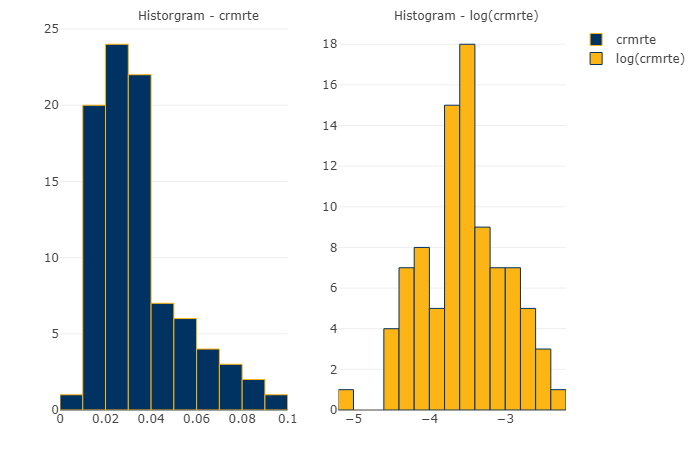
\includegraphics[width=0.9\textwidth,height=0.30\textheight]{images/EDA_histograms_crmrte.jpg}
		\caption{EDA : Histogram of CRMRTE and log(CRMRTE)}
		\label{fig:EDA Histogram CRMRTE}
	\end{subfigure}\vspace{3mm}% or \hspace{0.3\textwidth}
	
	\begin{subfigure}[b]{1.0\textwidth}
		\centering
		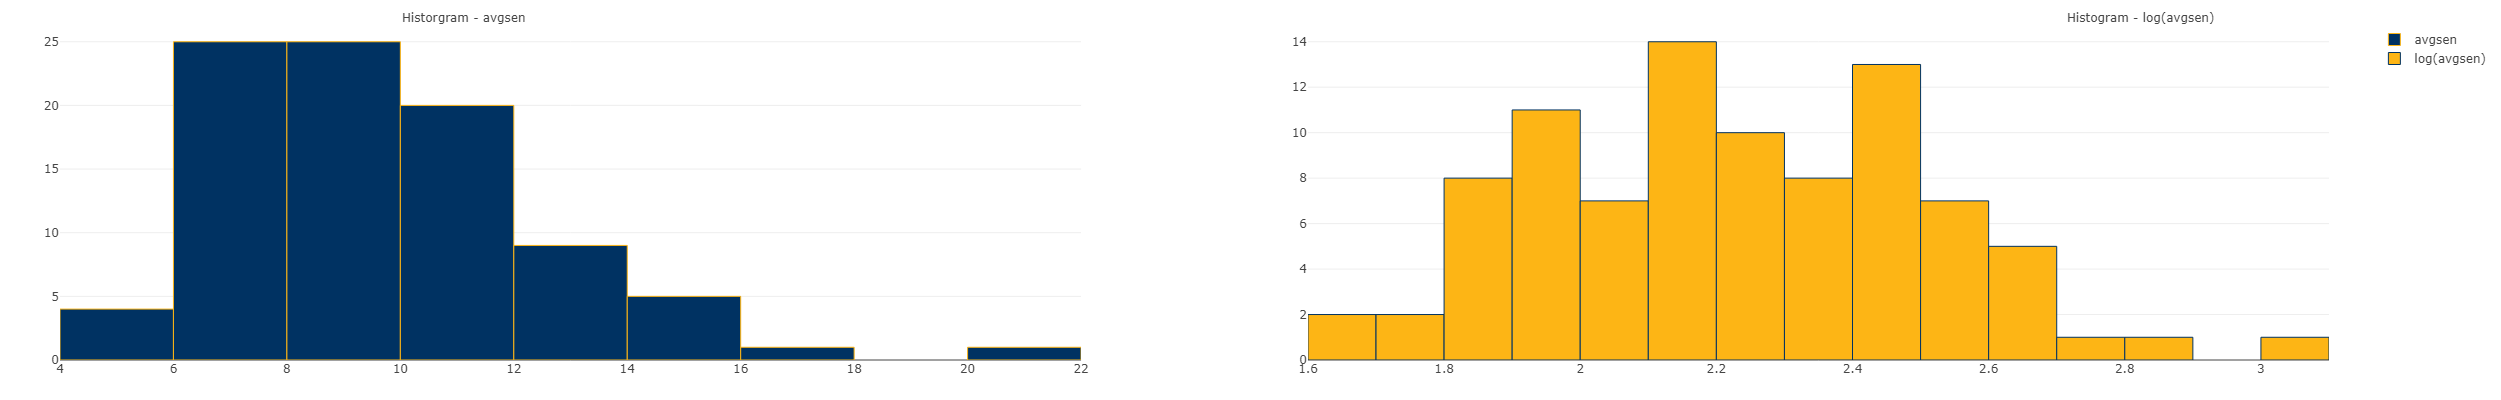
\includegraphics[width=0.9\textwidth,height=0.30\textheight]{images/EDA_histograms_avgsen.jpg}
		\caption{EDA : Histogram of AVGSEN and log(AVGSEN)}
		\label{fig:EDA Histogram AVGSEN}
	\end{subfigure}
	\label{fig:CRMRTE and AVGSEN Histogram}
	\caption{EDA : Distribution of Variables CRMRTE and AVGSEN}
\end{figure}

\pagebreak

\textbf{\textcolor{OrangeRed}{EXPLORATORY DATA ANALYSIS - CONTD.}}\\

Histograms Continued.\\

\begin{figure}[!ht]
	\begin{subfigure}[b]{1.0\textwidth}
		\centering
		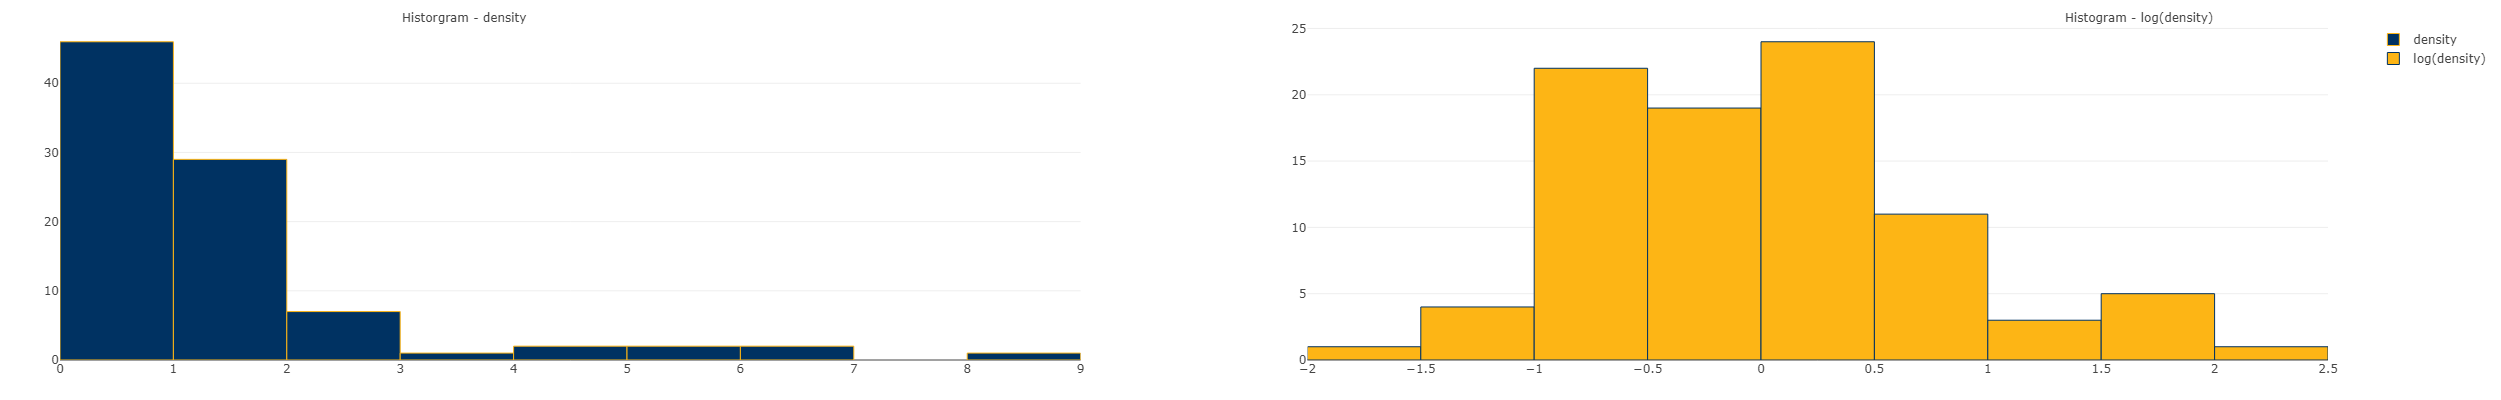
\includegraphics[width=0.9\textwidth,height=0.30\textheight]{images/EDA_histograms_density.jpg}
		\caption{EDA : Histogram of DENSITY and log(DENSITY)}
		\label{fig:EDA Histogram DENSITY}
	\end{subfigure}\vspace{3mm}% or \hspace{0.3\textwidth}
	
	\begin{subfigure}[b]{1.0\textwidth}
		\centering
		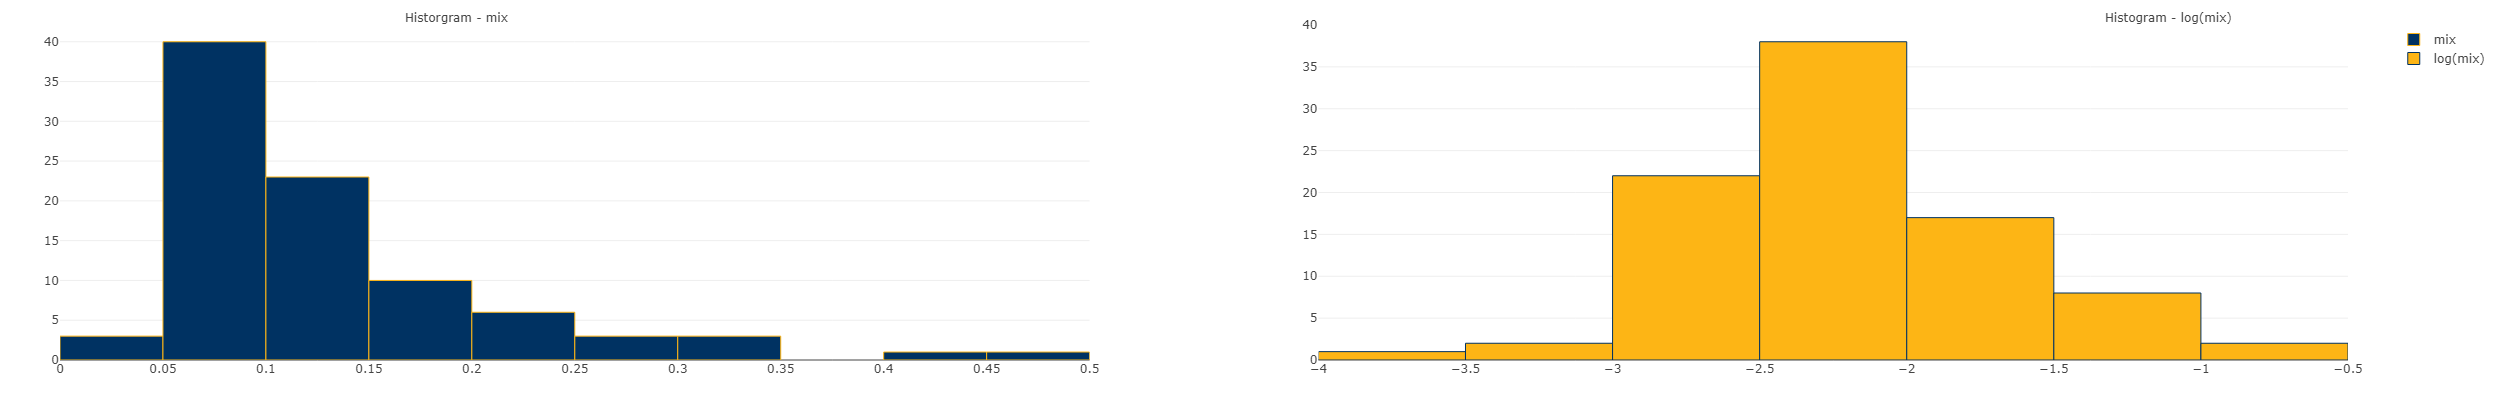
\includegraphics[width=0.9\textwidth,height=0.30\textheight]{images/EDA_histograms_mix.jpg}
		\caption{EDA : Histogram of MIX and log(MIX)}
		\label{fig:EDA Histogram MIX}
	\end{subfigure}
	\label{fig:DENSITY and MIX Histogram}
	\caption{EDA : Distribution of Variables DENSITY and MIX}
\end{figure}

\pagebreak

\textbf{\textcolor{OrangeRed}{EXPLORATORY DATA ANALYSIS - CONTD.}}\\

Histograms Continued.\\

\begin{figure}[!ht]
	\begin{subfigure}[b]{1.0\textwidth}
		\centering
		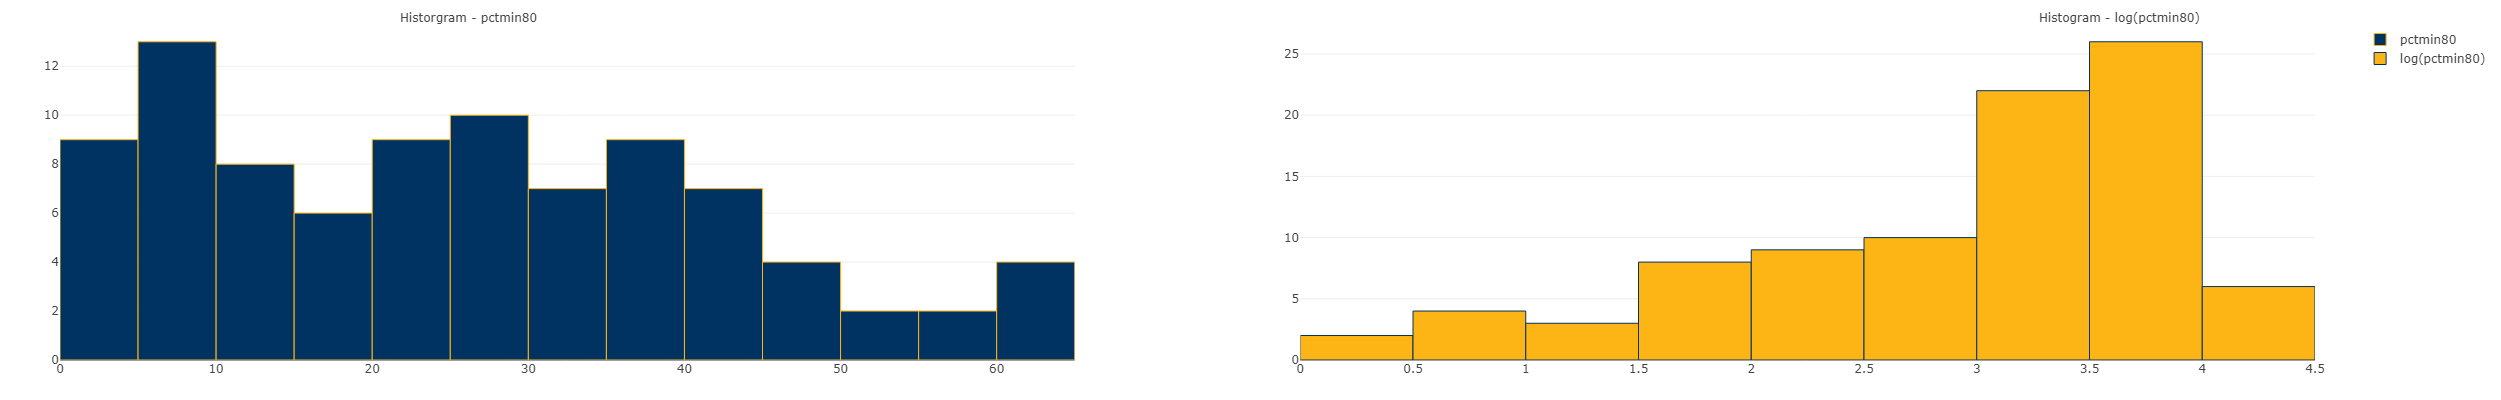
\includegraphics[width=0.9\textwidth,height=0.30\textheight]{images/EDA_histograms_pctmin80.jpg}
		\caption{EDA : Histogram of PCTMIN80 and log(PCTMIN80)}
		\label{fig:EDA Histogram PCTMIN80}
	\end{subfigure}\vspace{3mm}% or \hspace{0.3\textwidth}
	
	\begin{subfigure}[b]{1.0\textwidth}
		\centering
		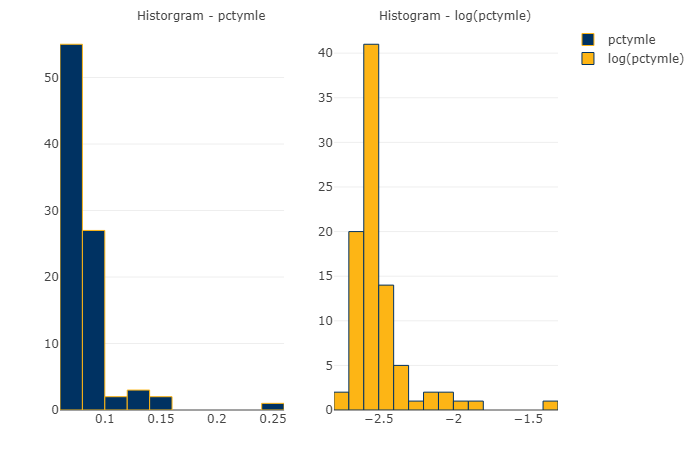
\includegraphics[width=0.9\textwidth,height=0.30\textheight]{images/EDA_histograms_pctymle.jpg}
		\caption{EDA : Histogram of PCTYMLE and log(PCTYMLE)}
		\label{fig:EDA Histogram PCTYMLE}
	\end{subfigure}
	\label{fig:PCTMIN80 and PCTYMLE Histogram}
	\caption{EDA : Distribution of Variables PCTMIN80 and PCTYMLE}
\end{figure}

\pagebreak

\textbf{\textcolor{OrangeRed}{EXPLORATORY DATA ANALYSIS - CONTD.}}\\

Histograms Continued.\\

\begin{figure}[!ht]
	\begin{subfigure}[b]{1.0\textwidth}
		\centering
		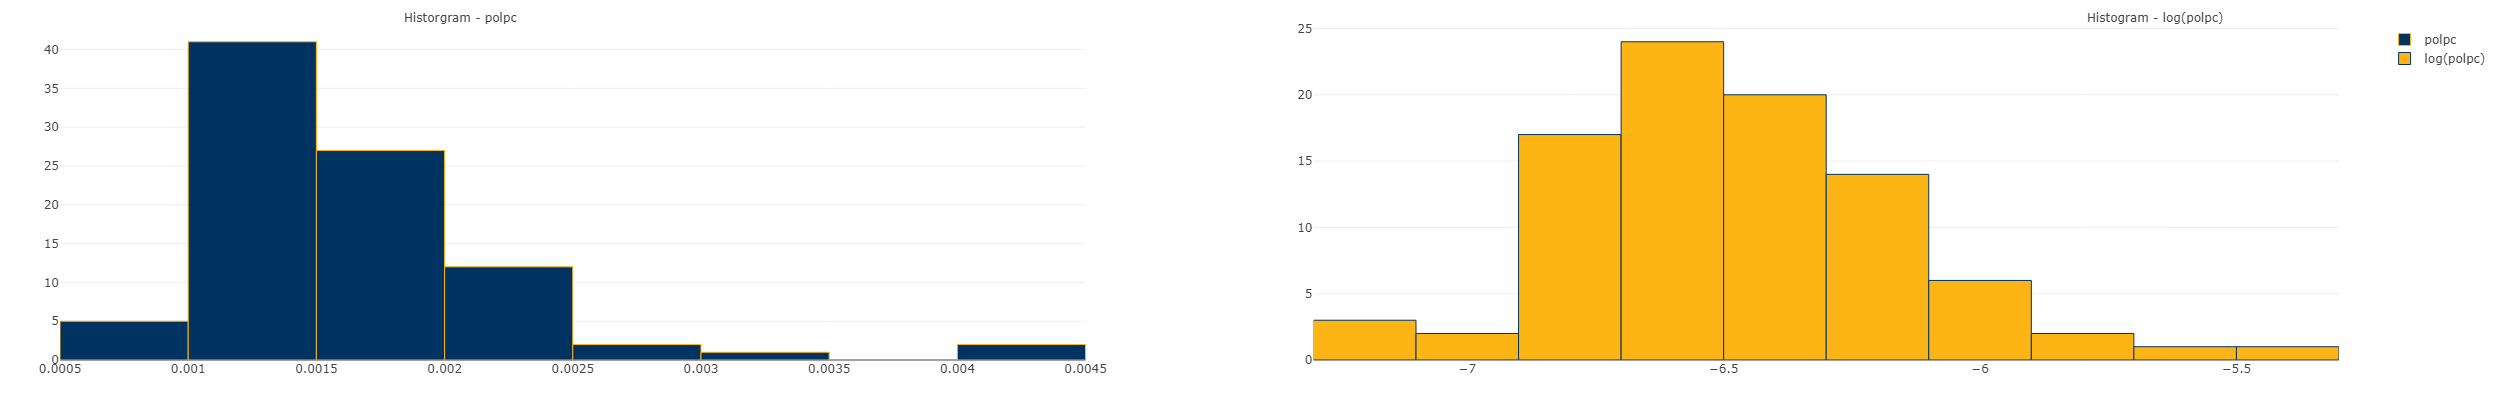
\includegraphics[width=0.9\textwidth,height=0.30\textheight]{images/EDA_histograms_polpc.jpg}
		\caption{EDA : Histogram of POLPC and log(POLPC)}
		\label{fig:EDA Histogram POLPC}
	\end{subfigure}\vspace{3mm}% or \hspace{0.3\textwidth}
	
	\begin{subfigure}[b]{1.0\textwidth}
		\centering
		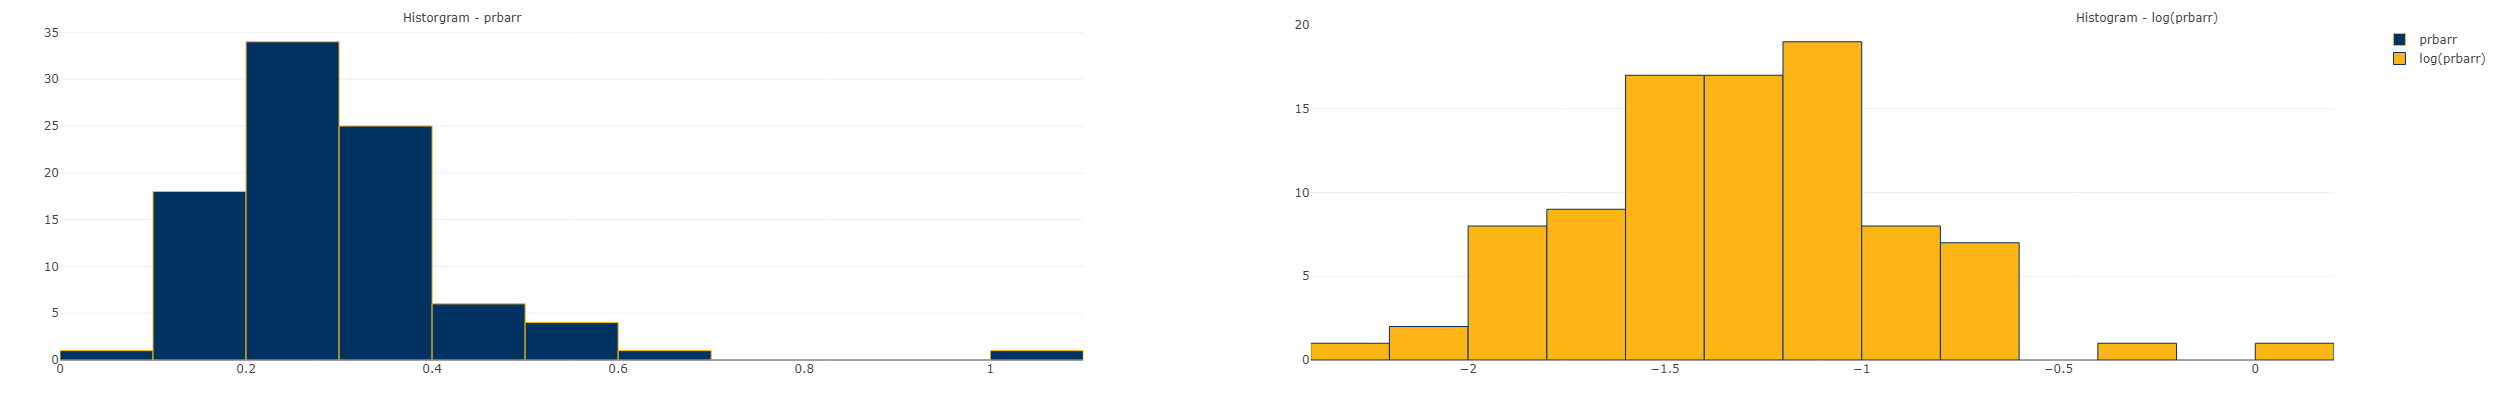
\includegraphics[width=0.9\textwidth,height=0.30\textheight]{images/EDA_histograms_prbarr.jpg}
		\caption{EDA : Histogram of PRBARR and log(PRBARR)}
		\label{fig:EDA Histogram PRBARR}
	\end{subfigure}
	\label{fig:POLPC and PRBARR Histogram}
	\caption{EDA : Distribution of Variables POLPC and PRBARR}
\end{figure}

\pagebreak

\textbf{\textcolor{OrangeRed}{EXPLORATORY DATA ANALYSIS - CONTD.}}\\

Histograms Continued.\\

\begin{figure}[!ht]
	\begin{subfigure}[b]{1.0\textwidth}
		\centering
		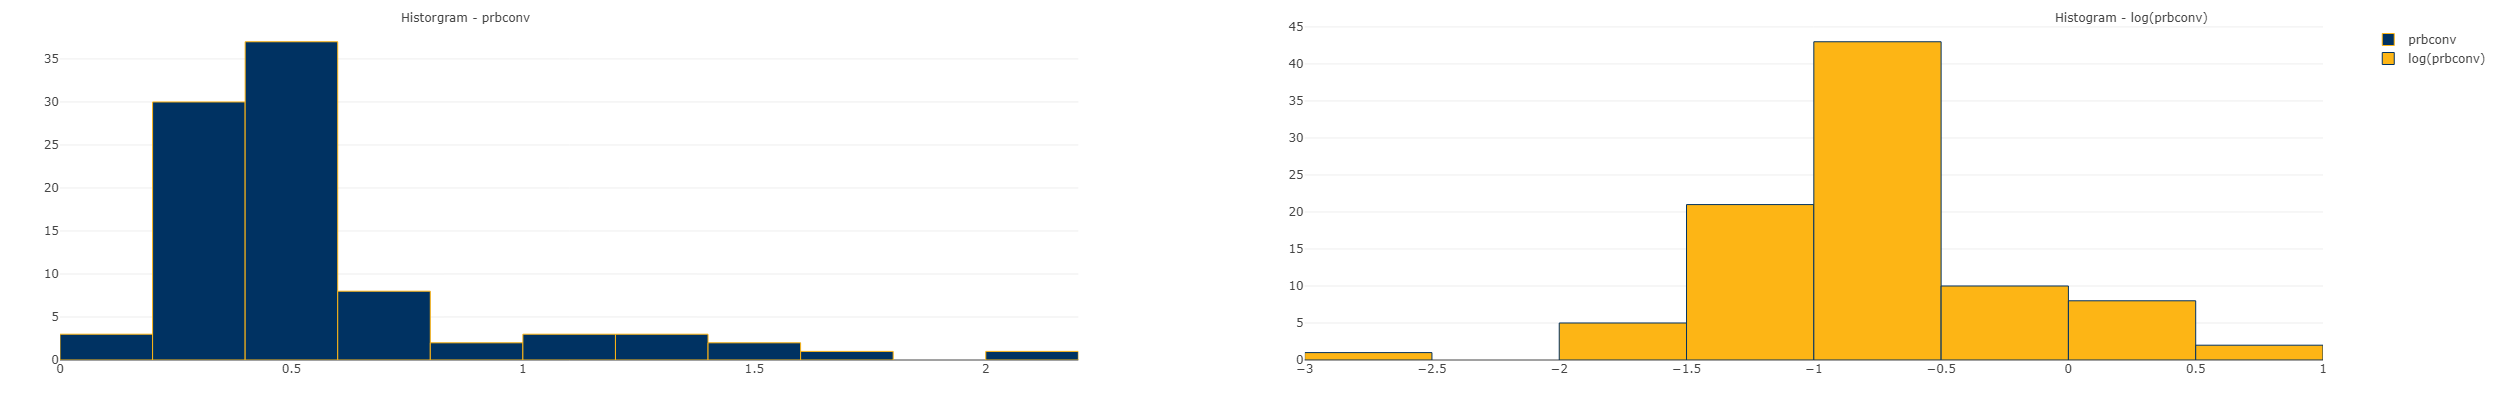
\includegraphics[width=0.9\textwidth,height=0.30\textheight]{images/EDA_histograms_prbconv.jpg}
		\caption{EDA : Histogram of PRBCONV and log(PRBCONV)}
		\label{fig:EDA Histogram PRBCONV}
	\end{subfigure}\vspace{3mm}% or \hspace{0.3\textwidth}
	
	\begin{subfigure}[b]{1.0\textwidth}
		\centering
		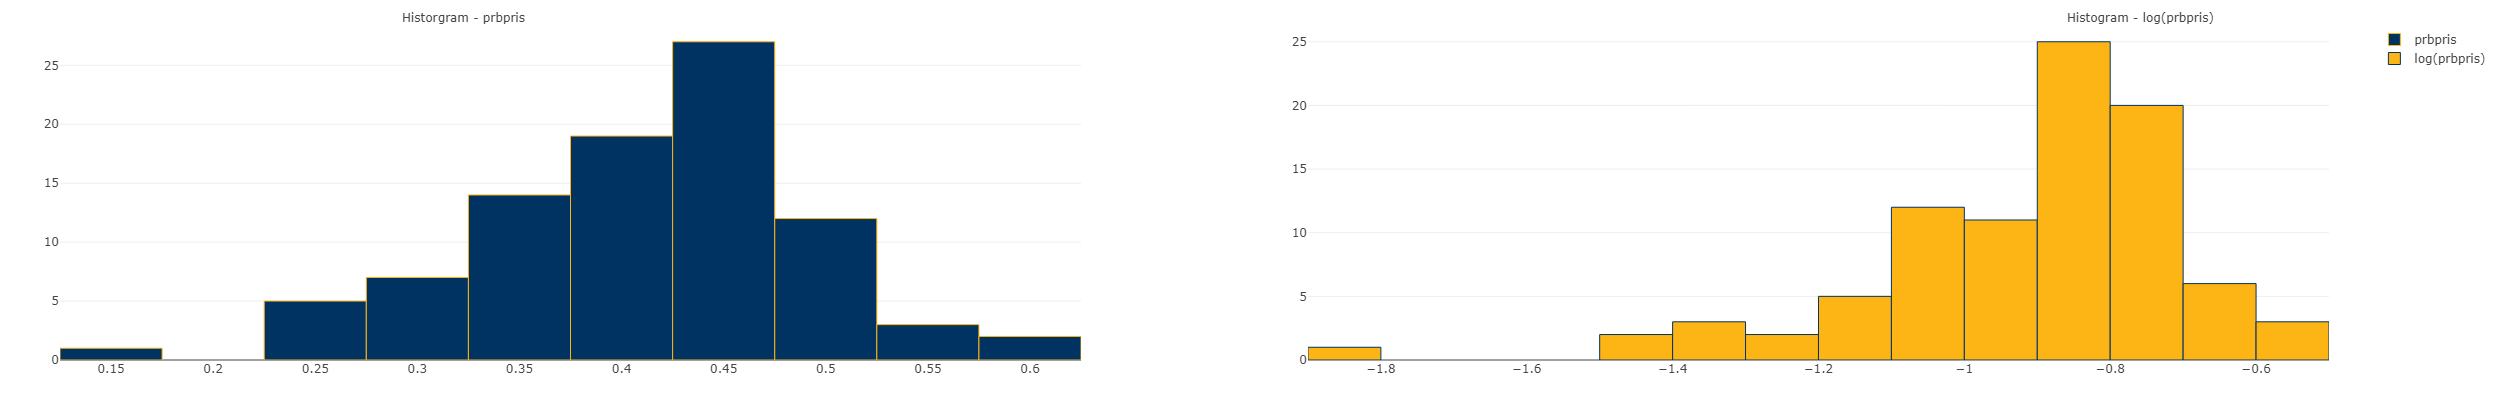
\includegraphics[width=0.9\textwidth,height=0.30\textheight]{images/EDA_histograms_prbpris.jpg}
		\caption{EDA : Histogram of PRBPRIS and log(PRBPRIS)}
		\label{fig:EDA Histogram PRBPRIS}
	\end{subfigure}
	\label{fig:PRBCONV and PRBPRIS Histogram}
	\caption{EDA : Distribution of Variables PRBCONV and PRBPRIS}
\end{figure}

\pagebreak

\textbf{\textcolor{OrangeRed}{EXPLORATORY DATA ANALYSIS - CONTD.}}\\

Histograms Continued.\\

\begin{figure}[!ht]
	\begin{subfigure}[b]{1.0\textwidth}
		\centering
		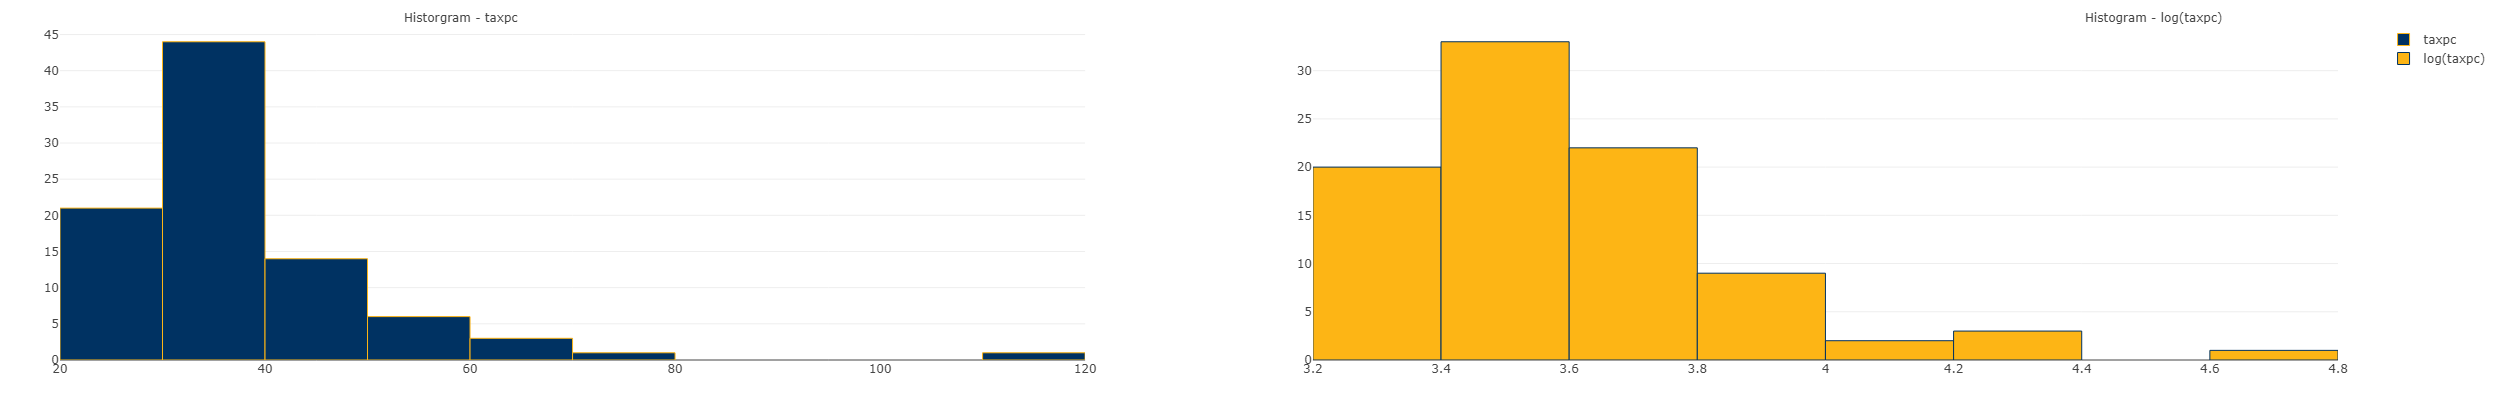
\includegraphics[width=0.9\textwidth,height=0.30\textheight]{images/EDA_histograms_taxpc.jpg}
		\caption{EDA : Histogram of TAXPC and log(TAXPC)}
		\label{fig:EDA Histogram TAXPC}
	\end{subfigure}\vspace{3mm}% or \hspace{0.3\textwidth}
	
	\begin{subfigure}[b]{1.0\textwidth}
		\centering
		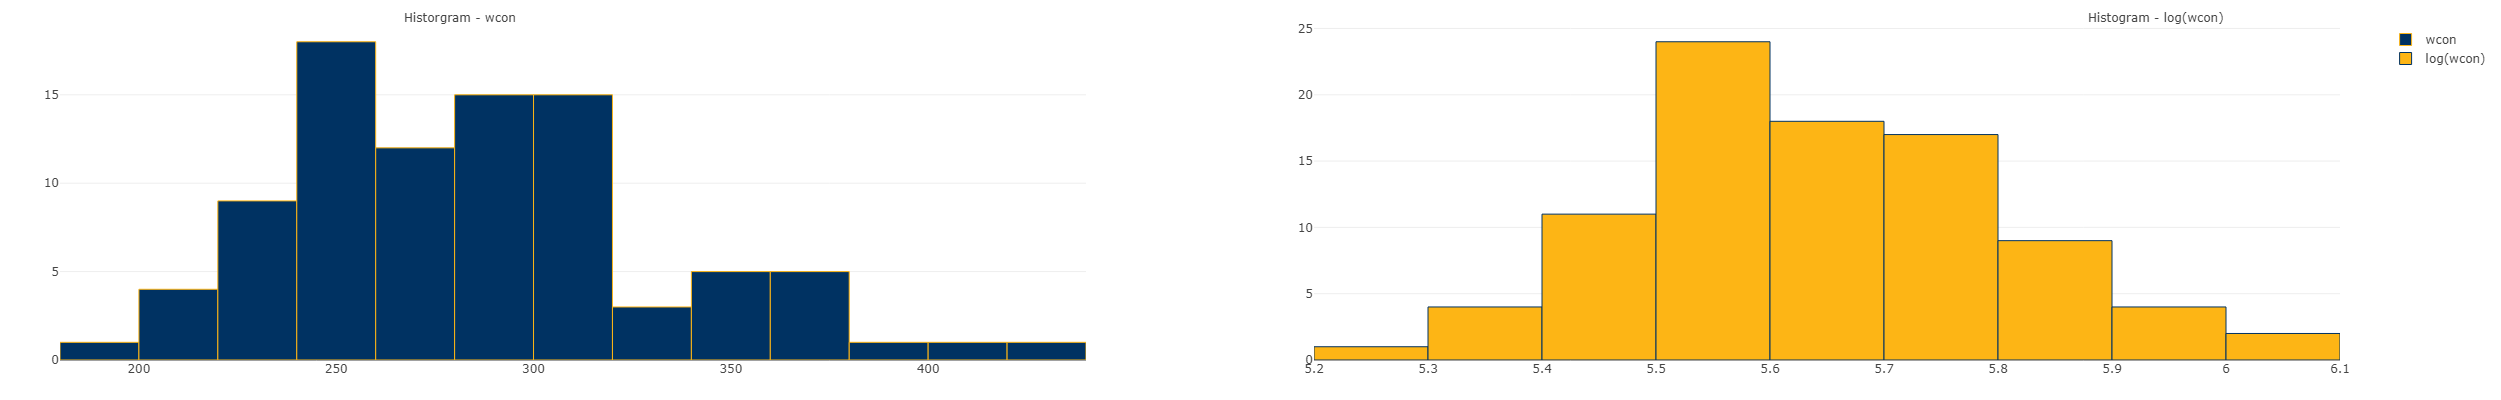
\includegraphics[width=0.9\textwidth,height=0.30\textheight]{images/EDA_histograms_wcon.jpg}
		\caption{EDA : Histogram of WCON and log(WCON)}
		\label{fig:EDA Histogram WCON}
	\end{subfigure}
	\label{fig:TAXPC and WCON Histogram}
	\caption{EDA : Distribution of Variables TAXPC and WCON}
\end{figure}

\pagebreak

\textbf{\textcolor{OrangeRed}{EXPLORATORY DATA ANALYSIS - CONTD.}}\\

Histograms Continued.\\

\begin{figure}[!ht]
	\begin{subfigure}[b]{1.0\textwidth}
		\centering
		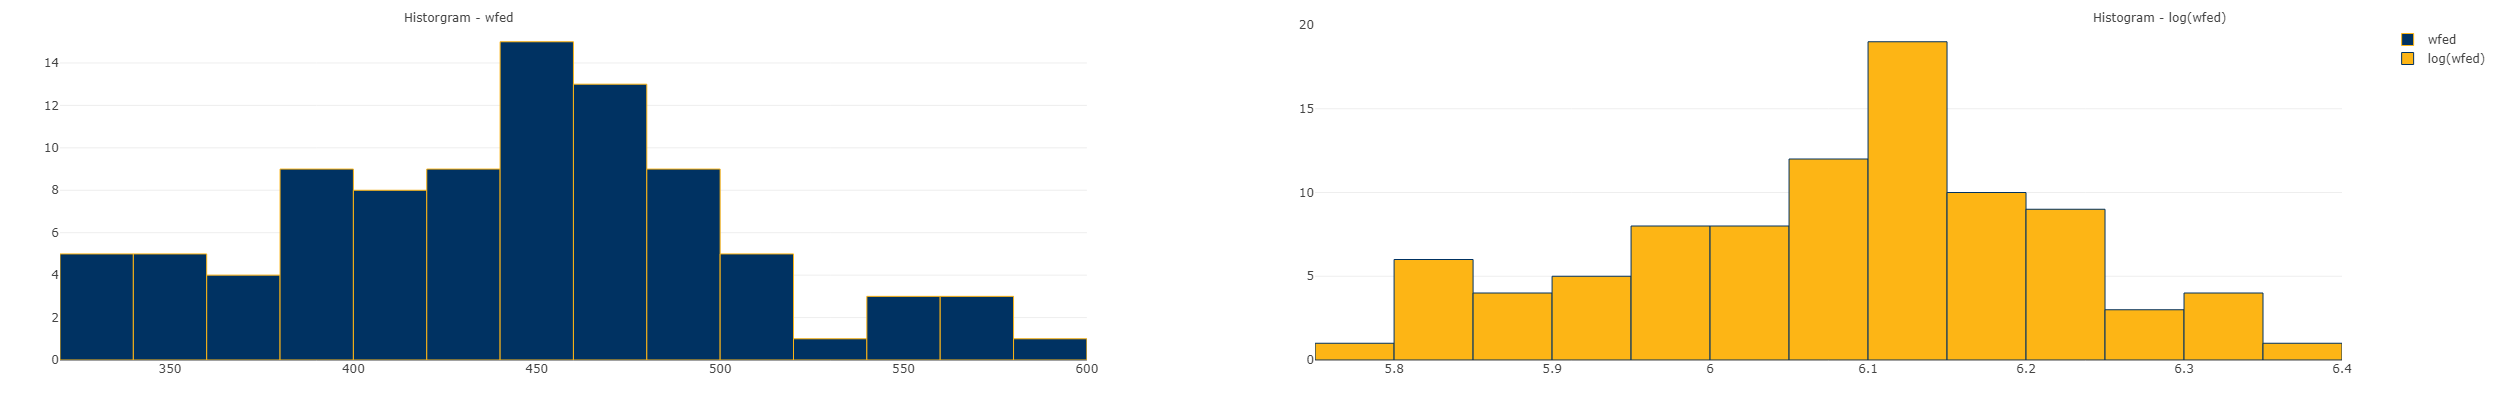
\includegraphics[width=0.9\textwidth,height=0.30\textheight]{images/EDA_histograms_wfed.jpg}
		\label{fig:EDA Histogram WFED}
		\caption{Histogram of WFED}
	\end{subfigure}\vspace{3mm}% or \hspace{0.3\textwidth}
	
	\begin{subfigure}[b]{1.0\textwidth}
		\centering
		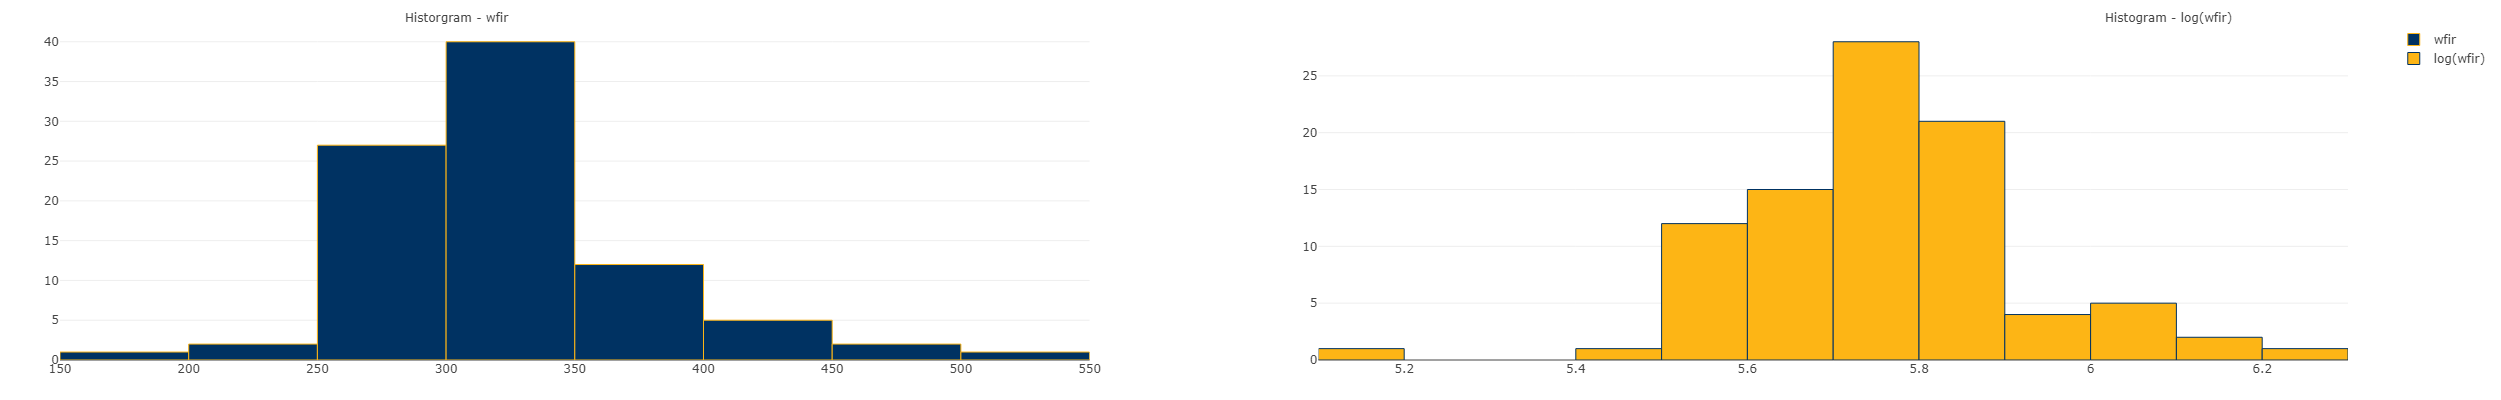
\includegraphics[width=0.9\textwidth,height=0.30\textheight]{images/EDA_histograms_wfir.jpg}
		\label{fig:EDA Histogram WFIR}
		\caption{Histogram of WFIR}
	\end{subfigure}
	\label{fig:WFED and WFIR Histogram}
	\caption{EDA : Distribution of Variables WFED and WFIR}
\end{figure}

\pagebreak

\textbf{\textcolor{OrangeRed}{EXPLORATORY DATA ANALYSIS - CONTD.}}\\

Histograms Continued.\\

\begin{figure}[!ht]
	\begin{subfigure}[b]{1.0\textwidth}
		\centering
		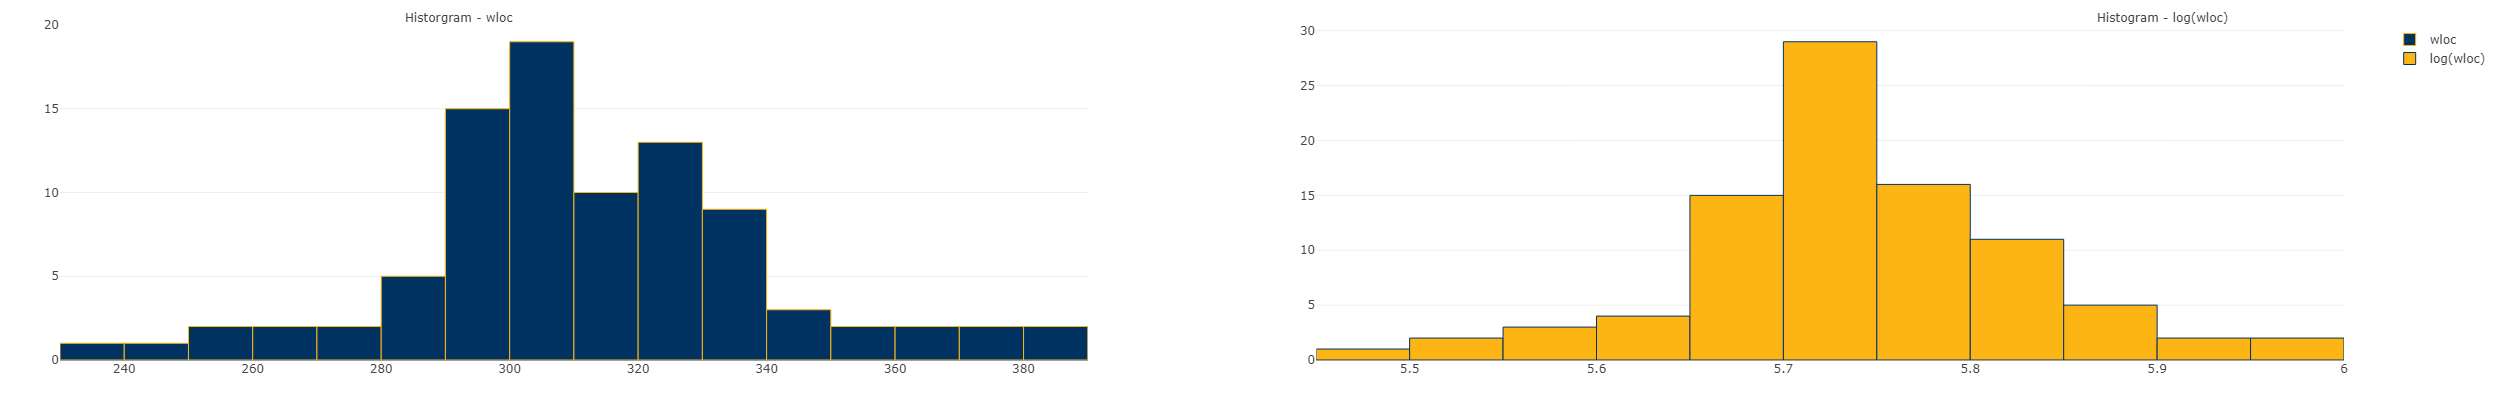
\includegraphics[width=0.9\textwidth,height=0.30\textheight]{images/EDA_histograms_wloc.jpg}
		\label{fig:EDA Histogram WLOC}
		\caption{Histogram of WLOC}
	\end{subfigure}\vspace{3mm}% or \hspace{0.3\textwidth}
	
	\begin{subfigure}[b]{1.0\textwidth}
		\centering
		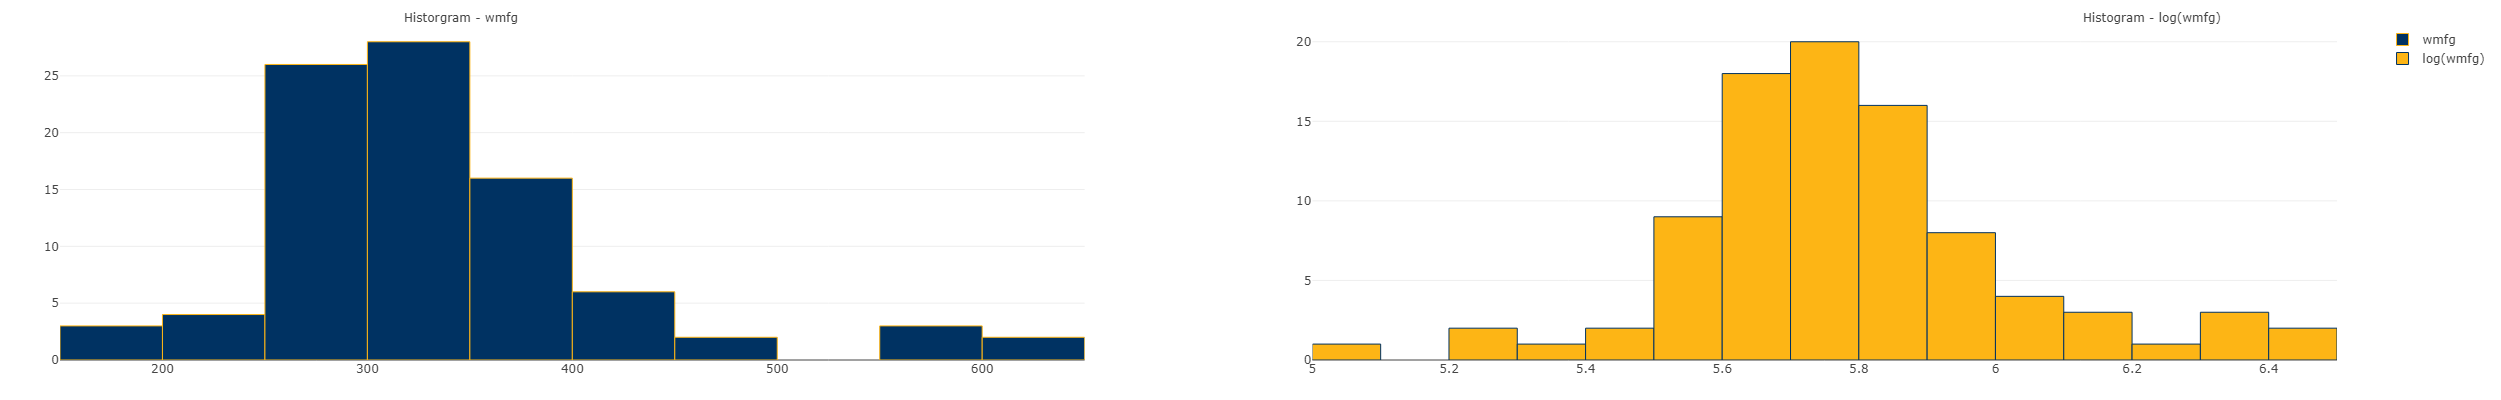
\includegraphics[width=0.9\textwidth,height=0.30\textheight]{images/EDA_histograms_wmfg.jpg}
		\label{fig:EDA Histogram WMFG}
		\caption{Histogram of WMFG}
	\end{subfigure}
	\label{fig:WLOC and WMFG Histogram}
	\caption{EDA : Distribution of Variables WLOC and WMFG}
\end{figure}

\pagebreak

\textbf{\textcolor{OrangeRed}{EXPLORATORY DATA ANALYSIS - CONTD.}}\\

Histograms Continued.\\

\begin{figure}[!ht]
	\begin{subfigure}[b]{1.0\textwidth}
		\centering
		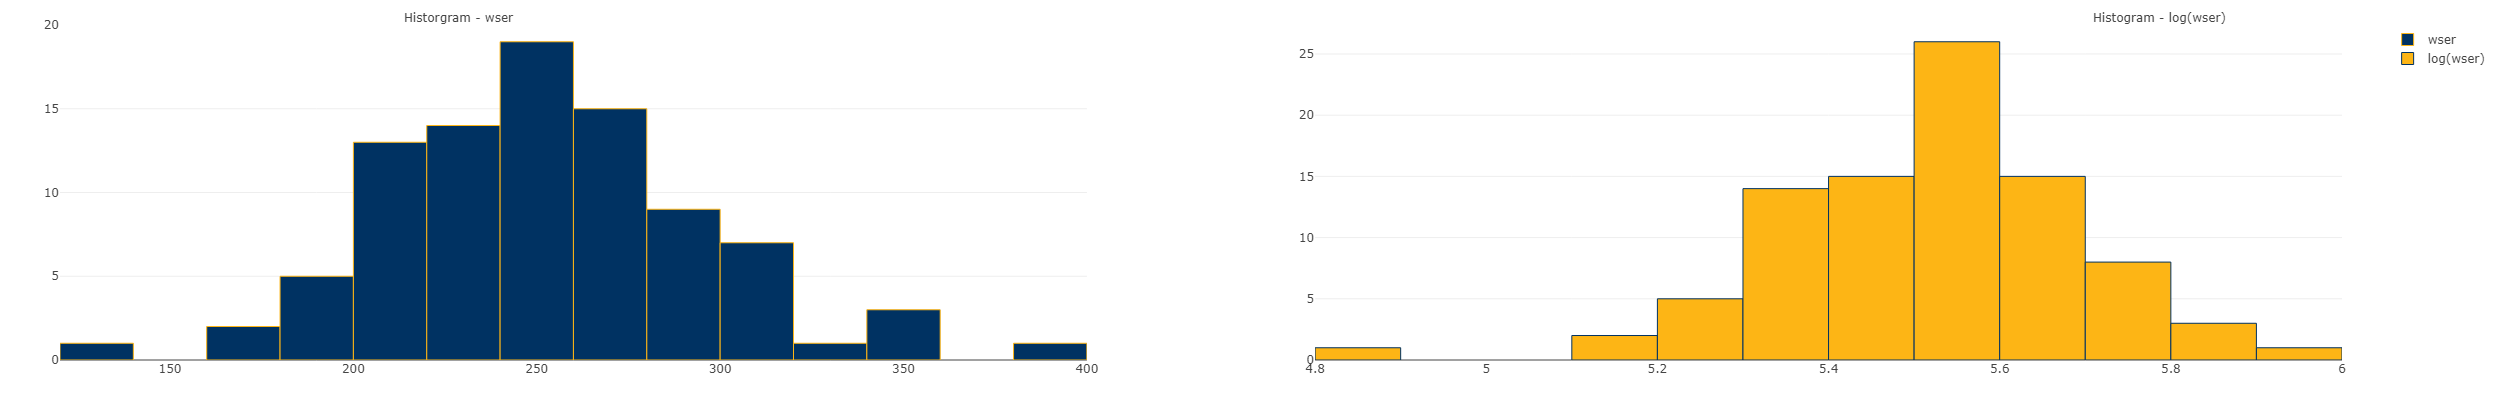
\includegraphics[width=0.9\textwidth,height=0.30\textheight]{images/EDA_histograms_wser.jpg}
		\label{fig:EDA Histogram WSER}
		\caption{Histogram of WSER}
	\end{subfigure}\vspace{3mm}% or \hspace{0.3\textwidth}
	
	\begin{subfigure}[b]{1.0\textwidth}
		\centering
		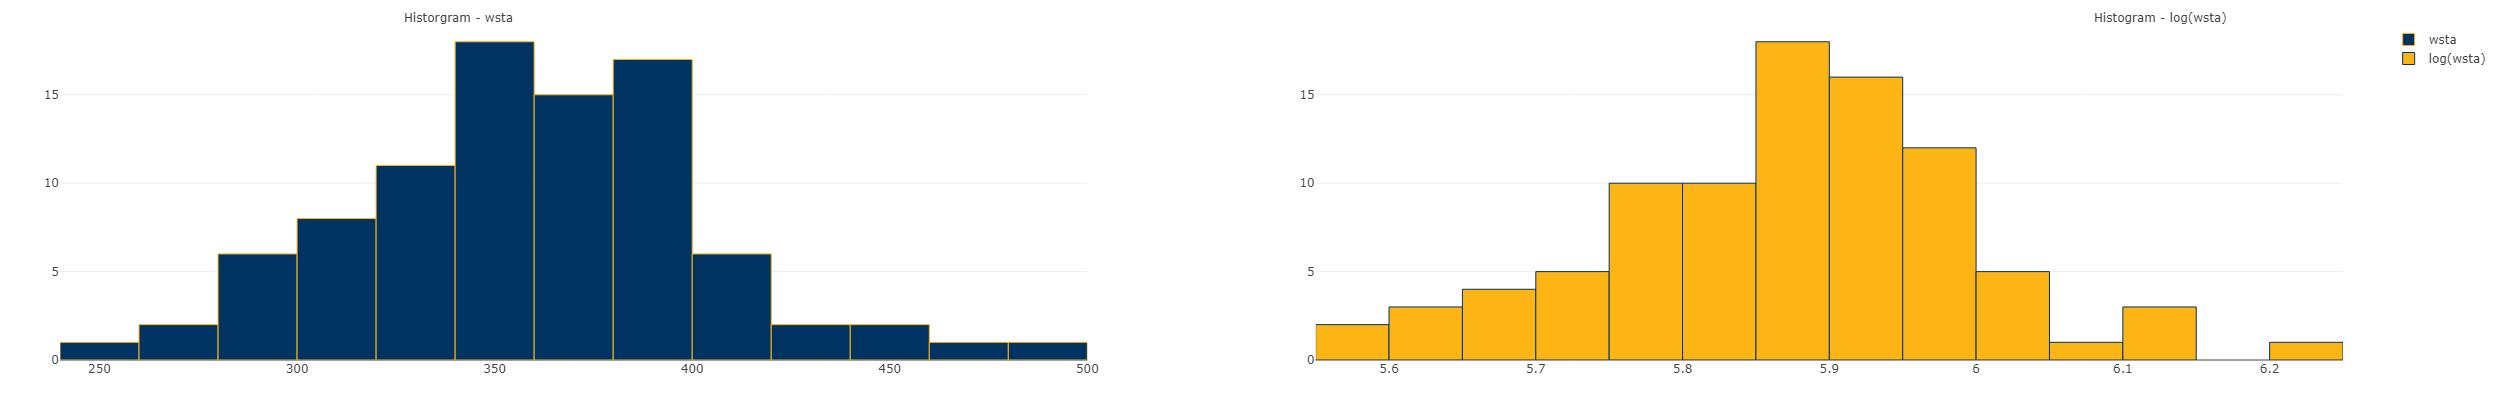
\includegraphics[width=0.9\textwidth,height=0.30\textheight]{images/EDA_histograms_wsta.jpg}
		\label{fig:EDA Histogram WSTA}
		\caption{Histogram of WSTA}
	\end{subfigure}
	\label{fig:WSER and WSTA Histogram}
	\caption{EDA : Distribution of Variables WSER and WSTA}
\end{figure}

\pagebreak

\textbf{\textcolor{OrangeRed}{EXPLORATORY DATA ANALYSIS - CONTD.}}\\

Histograms Continued.\\

\begin{figure}[!ht]
	\begin{subfigure}[b]{1.0\textwidth}
		\centering
		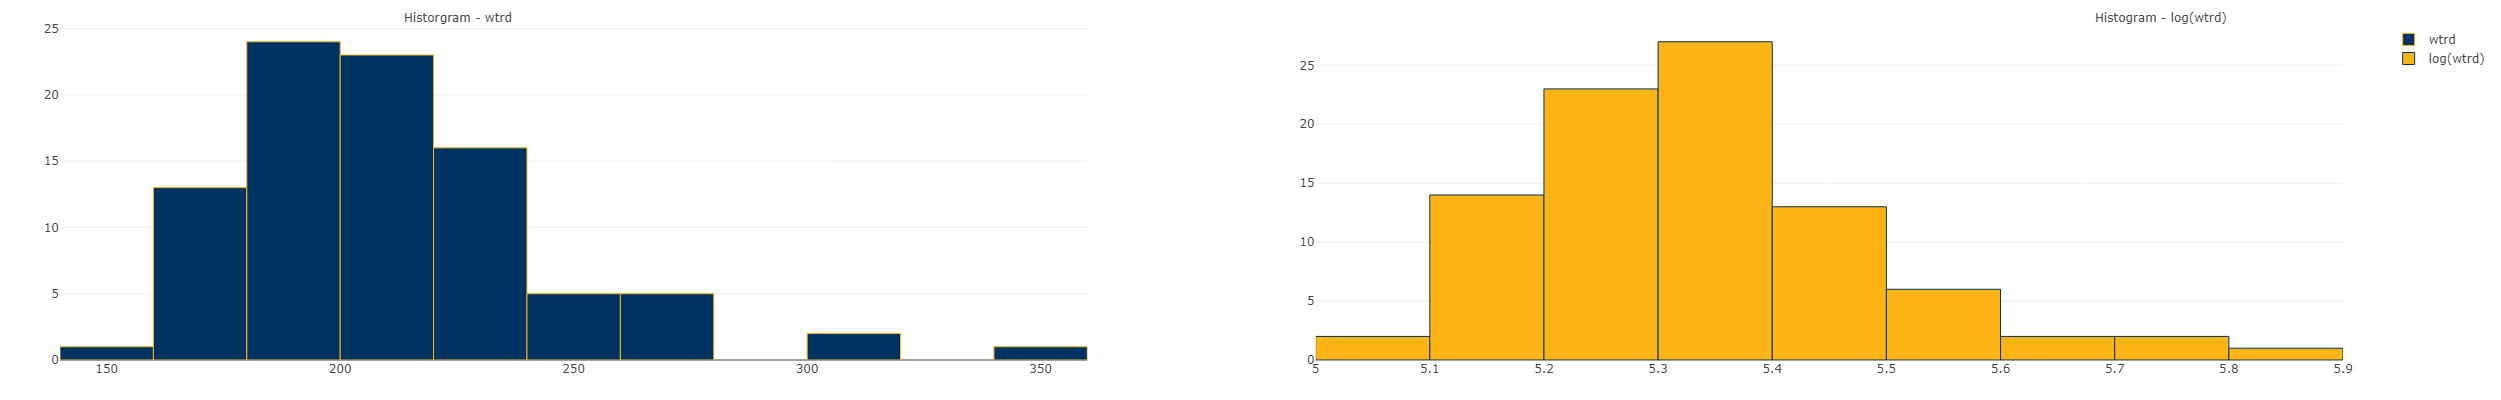
\includegraphics[width=0.9\textwidth,height=0.30\textheight]{images/EDA_histograms_wtrd.jpg}
		\label{fig:EDA Histogram WTRD}
		\caption{Histogram of WTRD}
	\end{subfigure}\vspace{3mm}% or \hspace{0.3\textwidth}
	
	\begin{subfigure}[b]{1.0\textwidth}
		\centering
		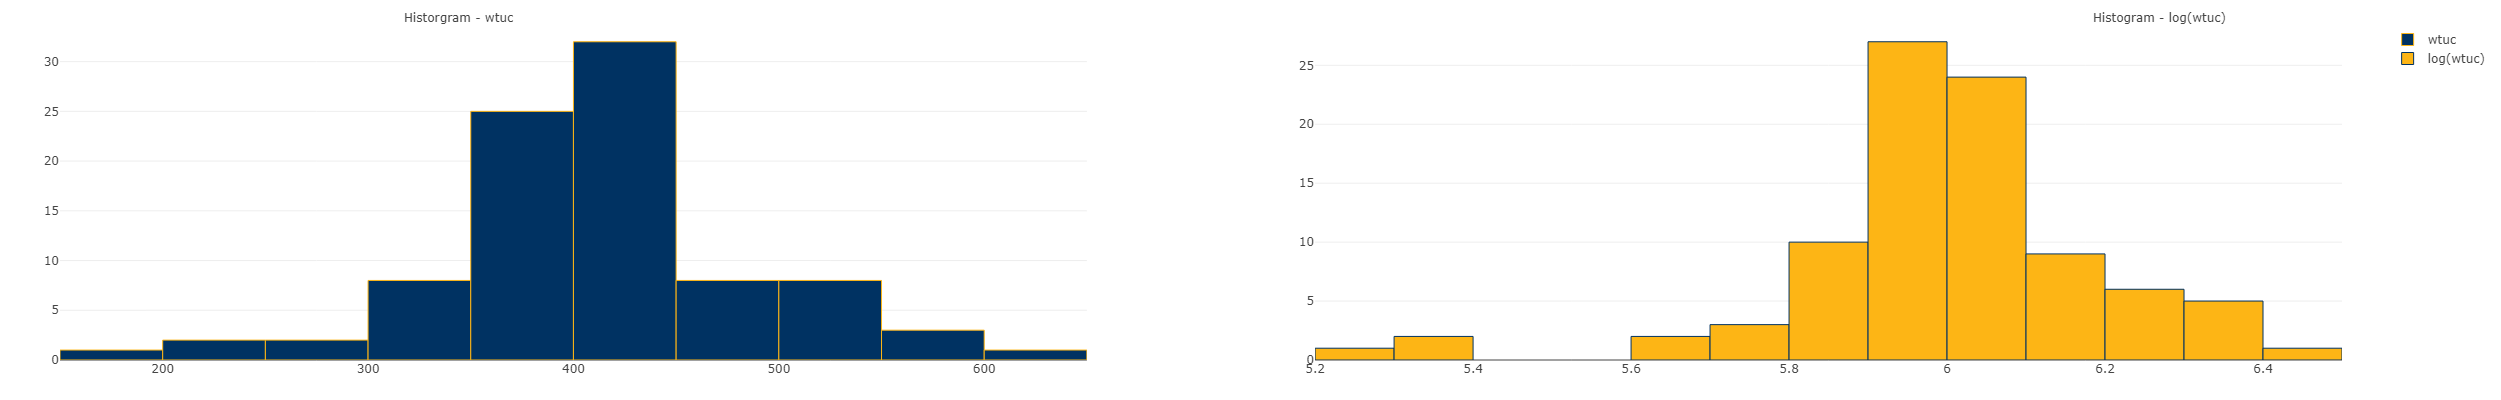
\includegraphics[width=0.9\textwidth,height=0.30\textheight]{images/EDA_histograms_wtuc.jpg}
		\label{fig:EDA Histogram WTUC}
		\caption{Histogram of WTUC}
	\end{subfigure}
	\label{fig:WTRD and WTUC Histogram}
	\caption{EDA : Distribution of Variables WTRD and WTUC}
\end{figure}

\pagebreak

%\textbf{\textcolor{OrangeRed}{EXPLORATORY DATA ANALYSIS - CONTD.}}\\
\section{Correlation}

We assess the correlation between dependent and independent variables, excluding all binary and identifier attributes.  Intersections where there exists a low statistical significance are removed from the plot to improve visibility of significant relationships.  There appears to be the strongest Pearson r correlation of the dependent variable $\textcolor{Blue}{crmrte}$ with potential regressors $\textcolor{Blue}{density}$ (0.73), $\textcolor{Blue}{wfed}$ (0.49), and $\textcolor{Blue}{polpc}$ (0.48).\\

Superficially, the relationship between $\textcolor{Blue}{polpc}$ and $\textcolor{Blue}{crmrte}$ seems as though it might be causal in the opposite direction - that is, the more crime present, the more police the county hires.  In this sense, $\textcolor{Blue}{polpc}$ might be better thought of as a dependent variable.\\

\begin{figure}[!ht]
	\centering
	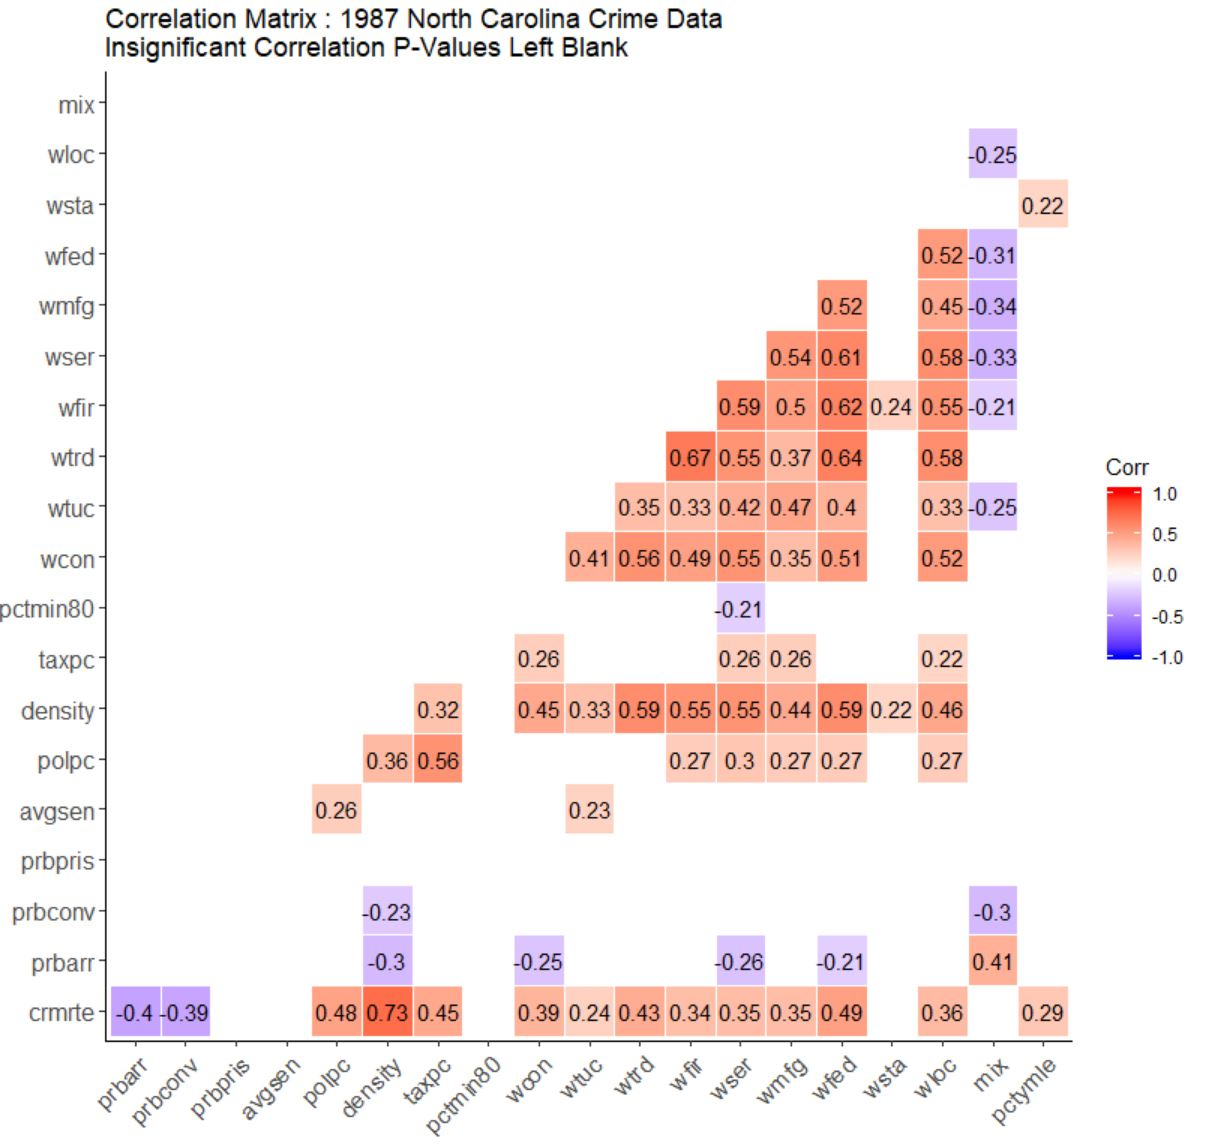
\includegraphics[width=0.9\textwidth]{images/EDA_correlation.jpg}
	\label{fig:EDA Correlation Matrix1}
	\caption{EDA : Correlation of Independent and Dependent Variables}
\end{figure}

\pagebreak

\textbf{\textcolor{OrangeRed}{EXPLORATORY DATA ANALYSIS - CONTD.}}\\

We also assess the correlation between log transforms of the variables of interest to assess the impact.  Feature intersections where there exists a low statistical significance are also removed from the plot for better visibility.  Generally, the impact is minimal to correlation between log and non-log transformed variables.\\

\begin{figure}[!ht]
	\centering
	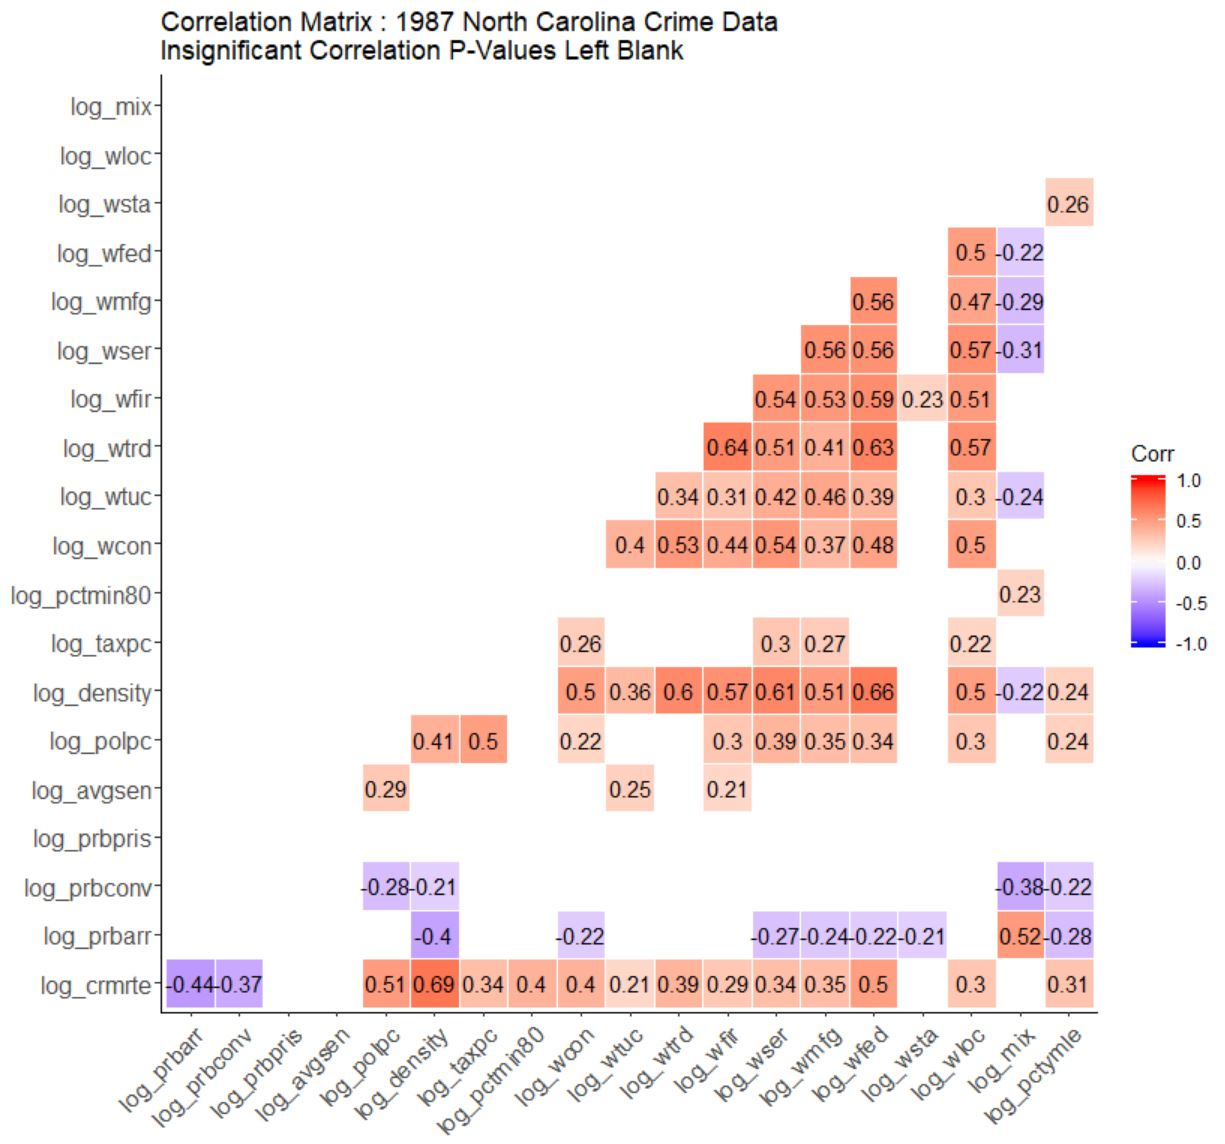
\includegraphics[width=0.9\textwidth]{images/EDA_log_correlation.jpg}
	\label{fig:EDA Correlation Matrix2}
	\caption{EDA : Correlation of Independent and Dependent Variables}
\end{figure}